\documentclass[12pt]{report}
\usepackage[utf8]{inputenc}
\usepackage{graphicx}
\usepackage{float}
\usepackage{listings}
\usepackage{titlesec}
\usepackage{xcolor}
\usepackage{fancyhdr}
\usepackage[pdfborder={0 0 0}]{hyperref} 
\usepackage{silence}
\usepackage{tikz}
\usepackage{charter}
\usepackage[table]{xcolor} 
\usepackage{float}  
\usepackage{longtable}          
\usepackage{atbegshi} 
\usepackage{url}
\usepackage{cellspace}
\usepackage[a4paper, left=1in, right=1in, bottom=0.8in, top=0.8in]{geometry}
\usepackage{tikz}
\usepackage{pgf-umlsd}
\newlength{\mymargin}
\setlength{\mymargin}{0.8cm}
\renewcommand{\baselinestretch}{1.4}
\pagenumbering{gobble}  % disable page numbering
\setlength{\cellspacetoplimit}{6pt}
\setlength{\cellspacebottomlimit}{6pt}
\usetikzlibrary{shapes.geometric, arrows}
% Draw border around page
\AtBeginShipout{%
  \AtBeginShipoutUpperLeft{%
    \begin{tikzpicture}[remember picture, overlay]
      \draw[line width=0.4pt] 
        ([xshift=\mymargin, yshift=\mymargin] current page.south west)
        rectangle 
        ([xshift=-\mymargin, yshift=-\mymargin] current page.north east);
    \end{tikzpicture}%
  }%
}
\setcounter{secnumdepth}{3}
\setcounter{tocdepth}{3}

\WarningsOff*
\definecolor{mybgcolor}{RGB}{73,83,101} % Dark bluish-gray
\lstdefinestyle{darkbash}{
    backgroundcolor=\color{mybgcolor},
    basicstyle=\ttfamily\color{white},
    frame=single,
    keywordstyle=\color{cyan},
    commentstyle=\color{gray},
}
\begin{document}

\begin{center}
	\begin{center}\begin{minipage}
			{0.1\textwidth}

			\centering
			\hspace*{-0.7cm}
			\includegraphics[width=2.2cm]{images/uni_logo.jpg}
		\end{minipage}%
		\hfill
		\begin{minipage}{0.7\textwidth}


			\centering
			\fontsize{12}{19}\selectfont % 14pt font with 18pt line spacing
			\textbf{People's Democratic Republic of Algeria} \\
			Ministry of Higher Education and Scientific Research \\
			\textbf{Martyr Hamma Lakhdar University of El Oued} \\

		\end{minipage}%
		\hfill
		\begin{minipage}{0.1\textwidth}

			\centering
			\includegraphics[width=2.2cm]{images/uni_logo.jpg}
		\end{minipage}
	\end{center}
	\vspace{0.5cm}
	\fontsize{12}{20}\selectfont
	Faculty of Exact Sciences \\
	Department of Computer Science \\
	\vspace{0.5cm}
	\textbf{Graduation Project Report} \\
	License 3rd And Final Year \\
	\rule{0.85\linewidth}{0.5pt} \\[0.3cm]
	\textbf{\Large Hospital Finder Mobile App}
	\rule{0.85\linewidth}{0.5pt}  \vspace{1cm}
	\begin{flushright}
		\begin{minipage}[t]{0.8\textwidth} % Total width of both columns
			\begin{minipage}[t]{0.48\textwidth}
				\hspace*{-1.7cm}
				\textbf{Prepared by:} \\[-7.7ex]
				\begin{itemize} \setlength\itemsep{0em}
					\setlength\itemsep{-0.8em}
					\setlength\labelsep{2cm}
					\setlength\labelwidth{0.5cm}
					\item \hspace*{-1.9cm} Gouder Hicham
					\item \hspace*{-1.9cm} Guedda Alla
					\item \hspace*{-1.9cm} Ayoub Zekri
				\end{itemize}

			\end{minipage}%
			\hfill
			\begin{minipage}[t]{0.48\textwidth}
				\hspace*{0.5cm}
				\textbf{Supervised by:} \\[-7.7ex]
				\begin{itemize} \setlength\itemsep{0em}
					\setlength\itemsep{-0.8em}
					\setlength\labelsep{-0.2cm}
					\setlength\labelwidth{0.5cm}
					\item \hspace*{0.3cm} Saci Medileh
				\end{itemize}
			\end{minipage}
		\end{minipage}
	\end{flushright}
	\vspace{5cm}
	\Large Academic Year: 2024/2025 \\
	\vfill
\end{center}
\tableofcontents
\newpage
\begin{center}
	\textbf{Abstract} \\
	\vspace*{0.3cm}
\end{center}

\noindent In regions like El Oued, private medical clinics, healthcare complexes, and hospitals are widespread, attracting patients from both within and outside the state. However, locating these facilities, determining the shortest routes, or finding accurate addresses remains a significant challenge, especially for visitors or those unfamiliar with the area. This difficulty often delays access to timely medical care. \vspace*{0.5cm}

\noindent To address this issue, we propose the development of a mobile application designed to provide the geographic locations of healthcare institutions in \textbf{El Oued}, with the potential for future expansion to other cities. \vspace*{0.5cm}

\noindent The app will offer detailed information about these facilities and integrate mapping services to assist users in navigation. Additionally, it may include a direct communication feature for inquiries and appointment scheduling. \vspace*{0.5cm}

\noindent By combining real-time location-based services with a user-friendly interface, the application aims to simplify the process of finding healthcare facilities, improve patient navigation, and enhance overall access to medical services. \vspace*{0.5cm}

\noindent \vspace*{0.5cm}\textbf{Keywords:} Mobile Application, Android, Geolocation, Google Maps.
\newpage
\begin{center}
	\textbf{Acknowledgment} \\
	\vspace*{0.3cm}
\end{center}

\noindent I would like to express my gratitude to everyone who contributed to the completion of this project. Their support and guidance played a significant role in its successful development.  \vspace*{0.5cm}

\noindent First, I extend my sincere appreciation to my supervisor, \textbf{Saci Medileh}, for his valuable guidance, feedback, and support throughout this work. his expertise and constructive advice have been essential in refining the project and addressing challenges effectively. \vspace*{0cm}

\noindent Furthermore, I sincerely thank the \textbf{professors of the Faculty of Exact Sciences} and it's memebers for their valuable insights and recommendations, which have helped improve the quality of this work.  \vspace*{0.5cm}

\noindent I also like to acknowledge the \textbf{administrative and technical staff} at the faculty for providing necessary resources and assistance throughout the process.  \vspace*{0.5cm}

\noindent Also, I appreciate the efforts of my colleagues, for their collaboration and commitment. Their contributions were crucial in different stages of the project, and their teamwork helped ensure its completion.  \vspace*{0.5cm}

\noindent Finally, I am grateful to my family for their continuous support and encouragement. Their patience and understanding allowed me to stay focused on this project.

\newpage

\addcontentsline{toc}{chapter}{General Introduction}










% ========================= ======================== = = = = 

\section*{\textbf{1. General Introduction}}
\rule{\linewidth}{1pt}  % Full-width horizontal line (adjust thickness if needed)


\addcontentsline{toc}{section}{1. Introduction}

\subsection*{\textbf{1.1 Project Presentation}}
\addcontentsline{toc}{subsection}{1.1 Project Presentation}

In today's fast-paced world, \textbf{access to healthcare services} is a fundamental need. However, finding the right hospital at the right time remains a \textbf{challenge} for many individuals. Whether it is for \textbf{emergency cases, routine check-ups, or specialized consultations}, people often struggle to locate nearby healthcare facilities that match their needs.

\noindent Traditional methods of searching for hospitals—such as \textbf{word-of-mouth recommendations or general internet searches}—are often \textbf{inefficient, time-consuming, and unreliable}. They rarely provide crucial details such as:
\begin{itemize}
	\item \textbf{Hospital specialties}
	\item \textbf{Available doctors and their expertise}
	\item \textbf{Operating hours and emergency services}
	\item \textbf{Real-time availability of services}
\end{itemize}

\noindent To address these challenges, we propose the development of a \textbf{Hospital Finder Mobile Application}. This app aims to help users \textbf{quickly and efficiently} locate nearby hospitals based on various criteria such as \textbf{location, specialty, available services, and real-time availability}. By integrating \textbf{modern technologies like geolocation, search filtering, and live data updates}, our system provides an \textbf{intelligent, user-friendly, and accessible solution} for patients and healthcare professionals.

\subsection*{\textbf{1.2 Application Objectives}}
\addcontentsline{toc}{subsection}{1.2 Application Objectives}

The primary goal of this application is to \textbf{simplify the process of finding hospitals and healthcare facilities} while ensuring users receive the most relevant and \textbf{real-time} information. Specifically, the application aims to:

\begin{itemize}
	\item \textbf{Improve Accessibility to Healthcare Services:} Provide an intuitive platform for users to locate hospitals, clinics, and medical specialists.
	\item \textbf{Enhance Patient Decision-Making:} Offer users hospital \textbf{ratings, available doctors, specialization areas, and real-time service availability}.
	\item \textbf{Reduce Search Time:} Optimize search and filtering functionalities to help users find the best hospital quickly.
	\item \textbf{Integrate Geolocation Services:} Enable real-time location tracking to suggest \textbf{the closest and most relevant medical facilities}.
	\item \textbf{Facilitate Patient-Hospital Communication:} Provide direct contact options such as \textbf{phone calls, appointment booking, and navigation assistance}.
\end{itemize}

\noindent By implementing these objectives, the \textbf{Hospital Finder Mobile Application} seeks to \textbf{enhance healthcare accessibility} and \textbf{reduce the time required to locate medical facilities}.

\subsection*{\textbf{1.3 Methodology and Adopted Formalisms}}
\addcontentsline{toc}{subsection}{1.3 Methodology and Adopted Formalisms}

To develop the \textbf{Hospital Finder Mobile Application}, we followed a structured approach, combining:
\begin{itemize}
	\item \textbf{Theoretical Study}
	\item \textbf{Technical Analysis}
	\item \textbf{Practical Implementation}
\end{itemize}

Our methodology consists of the following key steps:

\begin{enumerate}
	\item \textbf{Preliminary Study and Research}
	      \begin{itemize}
		      \item Analyze existing hospital-finder applications and their \textbf{limitations}.
		      \item Identify key \textbf{user needs and expectations} through research and surveys.
	      \end{itemize}

	\item \textbf{Requirement Specification and System Analysis}
	      \begin{itemize}
		      \item Define the \textbf{functional and non-functional requirements} of the system.
		      \item Develop \textbf{use case diagrams, system architecture, and database design} to ensure a structured implementation.
	      \end{itemize}

	\item \textbf{Design and Development}
	      \begin{itemize}
		      \item Implement a \textbf{cross-platform mobile application}.
		      \item Utilize \textbf{Flutter for the front-end} to ensure compatibility with both Android and iOS.
		      \item Store and manage data using \textbf{Firebase and a structured database modify later}.
	      \end{itemize}

	\item \textbf{Testing and Validation}
	      \begin{itemize}
		      \item Conduct rigorous \textbf{functionality, performance, and security} testing.
		      \item Gather \textbf{user feedback} and refine the app based on real-world usage.
	      \end{itemize}

	\item \textbf{Deployment and Future Enhancements}
	      \begin{itemize}
		      \item Deploy the application for public use, ensuring \textbf{a smooth user experience}.
		      \item Plan for \textbf{future updates}, including:
		            \begin{itemize}
			            \item \textbf{AI-based hospital recommendations modify later}
			            \item \textbf{Telemedicine features}
			            \item \textbf{Integration with electronic health records (EHR)}
		            \end{itemize}
	      \end{itemize}
\end{enumerate}









\newpage

\chapter{\textbf{Theoretical Study and Technical Choices}}
\rule{\linewidth}{1.5pt}

\section*{\textbf{1 Introduction}}
\addcontentsline{toc}{section}{Introduction}


In today's digital age, access to precise and reliable healthcare information is essential. Many existing applications provide hospital location services, but they often lack \textbf{detailed and accurate clinic information}.
This chapter explores the theoretical aspects of our \textbf{Hospital Finder Mobile Application}, analyzes existing solutions, and presents our improved approach.

\section*{\textbf{1 Preliminary Study}}
\addcontentsline{toc}{section}{1 Preliminary Study}

\vspace{-0.5cm}
\rule{7.5cm}{1.5pt}
\vspace{-0.5cm}
\subsection*{\textbf{1.1 Study of Existing Solutions: Geolocation, Search on Google Maps}}
\addcontentsline{toc}{subsection}{1.1 Study of Existing Solutions: Geolocation, Search on Google Maps}

Several solutions exist for finding hospitals and clinics, but they have \textbf{significant limitations}:

\begin{itemize}
	\item \textbf{Google Maps:}
	      Google Maps is the most widely used mapping service, offering general hospital searches. However, it \textbf{lacks precise information on clinics}, including doctors' availability, specialties, and operating hours.
	\item \textbf{Hospital Finder by Darshan University:}
	      This global application \textbf{only fetches hospital data from the Google Maps API} without allowing clinics to \textbf{add or modify their information}. Additionally, its \textbf{user interface is outdated}, making navigation difficult.
	\item \textbf{Local Availability:}
	      Currently, \textbf{no local application} provides a \textbf{dedicated hospital and clinic management system} that allows clinics to \textbf{register themselves, update details, and display real-time doctor availability}.
\end{itemize}

\subsection*{\textbf{1.2 Critique of Existing Solutions and Proposed Solution}}
\addcontentsline{toc}{subsection}{1.2 Critique of Existing Solutions and Proposed Solution}
\textbf{Limitations of Existing Solutions:}
\begin{itemize}
	\item No \textbf{custom clinic registration} or modifications
	\item Outdated UI and poor \textbf{user experience}
	\item No \textbf{detailed doctor profiles and schedules}
	\item Google Maps data is \textbf{too general} and lacks \textbf{localized clinic information}
	\item \textbf{Navigation issues} due to the absence of clear or guided paths to clinic locations, especially in certain areas
\end{itemize}

\noindent \textbf{Proposed Solution:}
To overcome these limitations, our \textbf{Hospital Finder Mobile Application} introduces:
\begin{itemize}
	\item \textbf{Enhanced Geolocation} → Provides \textbf{precise clinic locations} added by clinic administrators themselves.
	\item \textbf{Clinic Registration \& Management} → Clinics can \textbf{create, modify, and update their information}.
	\item \textbf{Detailed Doctor Profiles} → Displays \textbf{doctor specialties, working hours, availability, and schedules}.
	\item \textbf{Nearby Hospital \& Clinic Recommendations} → Suggests hospitals and clinics \textbf{based on real-time location}.
	\item \textbf{Integrated GPS \& Path Navigation} → Provides \textbf{step-by-step directions and map-based paths to each clinic}, addressing the issue of poor accessibility in some areas.
	\item \textbf{Modern UI \& Better User Experience} → A \textbf{new, intuitive, and visually appealing interface}.
\end{itemize}

\section*{\textbf{2 Conclusion}}
\addcontentsline{toc}{section}{2 Conclusion}

The existing hospital location solutions fail to provide \textbf{detailed, precise, and user-friendly} hospital and clinic information. Our \textbf{Hospital Finder Mobile Application} bridges this gap by offering:
\begin{itemize}
	\item A \textbf{better geolocation system} for \textbf{more accurate clinic placement}.
	\item The ability for \textbf{clinics to register and update their details}.
	\item \textbf{Comprehensive doctor profiles}, making hospital visits more efficient.
	\item \textbf{Map-based navigation with GPS}, enhancing access and ease of finding clinics.
	\item \textbf{A modern UI} with an intuitive design for easy navigation.
\end{itemize}

\noindent This enhanced system will significantly improve \textbf{healthcare accessibility} and provide a \textbf{better user experience} compared to existing solutions.











\newpage

\chapter{\textbf{Analysis and Specification of Requirements}}
\rule{\linewidth}{1.5pt}  % Full-width underline  

\section*{\textbf{1 Introduction}}
\addcontentsline{toc}{section}{1 Introduction}


\noindent To develop an efficient and user-friendly \textbf{Hospital Finder Mobile Application}, it is crucial to analyze the key actors involved, their roles, and the functional and non-functional requirements. This chapter presents an in-depth study of the application’s requirements and specifications.

\section*{\textbf{2 Global Analysis of the Application}}
\addcontentsline{toc}{section}{2 Global Analysis of the Application}

\noindent This section defines the main actors interacting with the system, along with their respective tasks and permissions. The application has four primary actors:
\begin{itemize}
	\item \textbf{User} – Searches for hospitals and doctors.
	\item \textbf{Clinic} – Registers doctors and manages clinic information.
	\item \textbf{Doctor} – View personal data and working hours .
	\item \textbf{Admin} – Approves new clinics and ensures system integrity.
\end{itemize}

\subsection*{\textbf{2.1 User Definition}}
\addcontentsline{toc}{subsection}{2.1 User Definition}
\noindent A \textbf{user} is a person who enters the application to access services such as searching for nearby clinics and doctors. Users do not need special registration and can quickly access relevant information.

\subsubsection*{\textbf{2.1.1 Main Tasks of a User}}
\addcontentsline{toc}{subsubsection}{2.1.1 Main Tasks of a User}

\begin{itemize}
	\item \textbf{Find Nearby Clinics:} View their locations on the map.
	\item \textbf{Find Available Doctors:} Check their specialties and schedules.
	\item \textbf{View Clinic Schedules:} Check the availability of clinics and doctors.
	\item \textbf{Contact Clinics:} Get phone numbers for appointments and inquiries.
\end{itemize}

\vspace{0.5cm}

\subsection*{\textbf{2.2 Clinic Definition}}
\addcontentsline{toc}{subsection}{2.2 Clinic Definition}

\noindent A \textbf{clinic} is an entity that registers in the application to add doctors and manage their data. Registration is not automatic; an admin must approve the clinic before it becomes active.

\subsubsection*{\textbf{2.2.1 Main Tasks of a Clinic}}
\addcontentsline{toc}{subsubsection}{2.2.1 Main Tasks of a Clinic}
\begin{itemize}
	\item \textbf{Enter Clinic Information:} Name, address, phone number, specialties.
	\item \textbf{Wait for Admin Approval:} The clinic remains inactive until approval.
	\item \textbf{Manage Doctors:} Once approved, the clinic can:
	      \begin{itemize}
		      \item Add doctors to the system.
		      \item Provide login credentials (email and password) to doctors.
	      \end{itemize}
\end{itemize}

\vspace{0.5cm}
\subsection*{\textbf{2.3 Doctor Definition}}
\addcontentsline{toc}{subsection}{2.3 Doctor Definition}
\noindent A \textbf{doctor} is a user who receives login credentials from the clinic they work at. Doctors cannot register independently but are added by their respective clinics.

\subsubsection*{\textbf{2.3.1 Doctor Tasks}}
\addcontentsline{toc}{subsubsection}{2.3.1 Doctor Tasks}
\begin{itemize}
	\item \textbf{Login:} Use the email and password provided by the clinic.
	\item \textbf{Check Schedule:} See availability and working hours. 
	\item \textbf{Check Personal Data:} View personal data and make sure patients have the correct information to get in contact or ask about them . 
\end{itemize}

\vspace{0.5cm}


\subsection*{\textbf{2.4 Admin Definition}}
\addcontentsline{toc}{subsection}{2.4 Admin Definition}

\noindent The \textbf{admin} is responsible for approving or rejecting newly registered clinics. They have a separate admin application to manage the system efficiently.

\subsubsection*{\textbf{2.4.1 Admin Tasks}}
\addcontentsline{toc}{subsubsection}{2.4.1 Admin Tasks}
\begin{itemize}
	\item \textbf{Review Clinic Registration Requests:} Check clinic information for validity.
	\item \textbf{Approve or Reject Clinics:} Grant or deny access based on verification.
	\item \textbf{Review User Reports:} Check reports made by users and decide to ignore it or take action.
	\item \textbf{Suspend / Delete Clinic Account:} Admin can suspend or deleted clinic account if clinic is reported multiple times. 
	\item \textbf{Ensure System Integrity:} Monitor and manage the overall platform.
\end{itemize}


\subsection*{2.5 App Users Information Table}
\addcontentsline{toc}{subsection}{2.5 App Users Information Table}
\noindent The application collects specific information for each user type to support functionality, access control, and communication. Each user type—whether a patient, clinic, doctor, or admin—has a tailored set of required details that align with their role in the system. The table below outlines the key types of users in the application and the information stored for each to facilitate registration, authentication, and system interaction.
\vspace{0.3cm}
\begin{table}[H]
	\centering
	\renewcommand{\arraystretch}{1.3}
	\begin{tabular}{|p{4cm}|p{11.5cm}|}
		\hline
		\rowcolor[HTML]{C0C0C0}
		\textbf{User Type}                     & \textbf{Stored Information}                                       \\
		\hline

		\hspace{0.5cm}\textbf{Patient / Guest} &
		Full name, email, password, Google Login id, notification preferences.                                     \\
		\hline

		\hspace{1.4cm}\textbf{Clinic}          &
		Clinic name, email, password, phone number, address, location coordinates, registration number and images. \\
		\hline

		\hspace{1.4cm}\textbf{Doctor}          &
		Full name, email, phone number, associated clinic and specialty, availability schedule.                    \\
		\hline

		\hspace{1.4cm}\textbf{Admin}           &
		Email and password only, used for platform management access.                                              \\
		\hline
	\end{tabular}
	\begin{center}
		\vspace{0.5cm}
		\textit{\textbf{Figure: App user types and the information they store.}}
	\end{center}
\end{table}


\newpage
\subsection*{2.6 App Users Roles Table}
\addcontentsline{toc}{subsection}{2.6 App Users Roles Table}	
\noindent The application consists of multiple user roles, each with distinct responsibilities and functionalities. Understanding these roles is essential for ensuring smooth operation and proper management within the system. Below is a breakdown of the key roles and their main tasks:
\vspace{0.2cm}
% Longtable for splitting across pages
\renewcommand{\arraystretch}{1.3} % Adjust row spacing

\begin{longtable}{|p{3cm}|p{6cm}|p{6cm}|}

	\hline
	\rowcolor[HTML]{C0C0C0}
	\hspace*{1cm}\textbf{Role}                                                                                 & \hspace*{1.9cm} \textbf{Definition}                                                 & \hspace*{1.9cm}\textbf{Main Tasks} \\
	\hline
	\endfirsthead

	\hline
	\rowcolor[HTML]{C0C0C0}
	\hspace*{1cm}\textbf{Role}                                                                                 & \hspace*{1.9cm} \textbf{Definition}                                                 & \hspace*{1.9cm}\textbf{Main Tasks} \\
	\hline
	\endhead

	\hspace*{0.1cm}\textbf{User (Patient)}                                                                     & A person accessing the app to find clinics and doctors without registration.        &
	• Search for nearby clinics and doctors.\newline
	• View doctor specialties and clinic details.\newline
	• Check clinic and doctor schedules.\newline
	• Contact clinics for appointments.                                                                                                                                                                                                   \\
	\hline

	\hspace*{0.9cm}\textbf{Clinic}                                                                             &
	An entity that registers on the app to manage doctors and provide services. Approval by admin is required. &
	• Register and provide clinic details.\newline
	• Wait for admin approval.\newline
	• Add and manage doctors.\newline
	• Provide login credentials to doctors.                                                                                                                                                                                               \\
	\hline


	\hspace*{0.85cm}\textbf{Doctor}                                                                            & A medical professional registered under a clinic who cannot independently sign up.  &
	• Log in with clinic-provided credentials.\newline
	• View their schedule.\newline
	• View their personal data.                                                                                                                                                                                            \\
	\hline

	\hspace*{0.85cm}\textbf{Admin}                                                                             & The system manager responsible for approving clinics and ensuring smooth operation. &
	• Review and approve/reject clinic registrations.\newline
	• Review Reports.\newline   
	• Suspend/Delete Clinic Account.                                                                                                                                                   \\
	\hline
\end{longtable}
\begin{center}
	\textit{\textbf{Figure: App user roles and desception.}}
\end{center}


\subsection*{2.6 Conclusion}
\addcontentsline{toc}{subsection}{2.6 Conclusion}
This document has provided an overview of the system, focusing on the roles and responsibilities of users. The Hospital Finder Mobile App ensures smooth interaction between patients, clinics, and administrators.
\vspace{0.5cm}
\section*{\textbf{3 Functional Requirements Specification}}
\addcontentsline{toc}{section}{3 Functional Requirements Specification}

\noindent The functional requirements define the expected behavior of the application. These include:

\begin{itemize}
	\item \textbf{User Authentication:} Clinics, doctors, and admins must log in securely.
	\item \textbf{Geolocation Services:} Users can find nearby clinics and doctors with precise locations.
	\item \textbf{Clinic and Doctor Management:} Clinics can add doctors, and update their availability.
	\item \textbf{Admin Panel:} The admin can approve or reject clinic registrations and user reports and also can delete or suspent Clinic account.
\end{itemize}

\section*{\textbf{4 Non-Functional Requirements Specification}}
\addcontentsline{toc}{section}{4 Non-Functional Requirements Specification}
\noindent The non-functional requirements define the application's quality attributes, such as performance, security, and usability.

\begin{itemize}
	\item \textbf{Performance:} The application should provide quick search results with minimal load time.
	\item \textbf{Security:} User data must be encrypted, and authentication should be secure.
	\item \textbf{Scalability:} The system should handle a growing number of users and clinics efficiently.
	\item \textbf{User-Friendly Interface:} The UI should be intuitive and responsive across all devices.
\end{itemize}


\section*{\textbf{5 Use Case Diagrams}}
\addcontentsline{toc}{section}{5 Use Case Diagrams}
\rule{0.45\linewidth}{0.7pt}
\subsection*{\textbf{5.1 Definition of Use Case Diagrams}}
\addcontentsline{toc}{subsection}{5.1 Definition of Use Case Diagrams}


\noindent A \textbf{Use Case Diagram} is a visual representation that describes the interactions between users (actors) and the system. It outlines the different functionalities provided by the application and the roles of each user in relation to those functionalities.

\noindent These diagrams are part of \textbf{Unified Modeling Language (UML)} and help in understanding how users engage with the application. The primary components of a use case diagram include:

\begin{itemize}
	\item \textbf{Actors:} Represent users or external systems interacting with the application.
	\item \textbf{Use Cases:} Define specific actions that users can perform in the system.
	\item \textbf{Associations:} Indicate the relationship between actors and their use cases.
	\item \textbf{System Boundary:} Defines the scope of the application by enclosing all the use cases.
\end{itemize}

\noindent The goal of these diagrams is to **provide a clear, high-level understanding** of how different actors interact with the system’s functionalities, making it easier for developers, stakeholders, and designers to visualize and refine the system requirements.

\subsection*{\textbf{5.2 Use Case Diagrams for the Application}}
\addcontentsline{toc}{subsection}{5.2 Use Case Diagrams for the Application}


\noindent Below are the key \textbf{Use Case Diagrams} representing interactions for different roles in the \textbf{Hospital Finder Mobile Application}.

\newpage
\subsubsection*{\textbf{5.2.1 Doctor Interactions}}
\addcontentsline{toc}{subsubsection}{5.2.1 Doctor Interactions}
The following diagram illustrates how a doctor interacts with the application. Doctors have limited access and can only perform actions related to their schedules and their data.

\vspace{0.5cm}

\noindent \textbf{Observation:} In this and other diagrams, the element \textbf{ \texttt{<<abstract>> Do/ask Server}} acts as a unified layer for all communication between the app and backend.\textbf{"Do"} refers to sending commands to perform actions, while \textbf{"Ask"} refers to requesting information. This abstraction centralizes operations like in this diagram example: View Data which is a sending a request to our \textbf{App's Server/Database} and managing into one scalable points, keeping diagrams clean and consistent.



\vspace{0.5cm}
\noindent \textbf{• Use Case Diagram: Doctor Using the App}
\vspace{0.6cm}
\begin{center}
	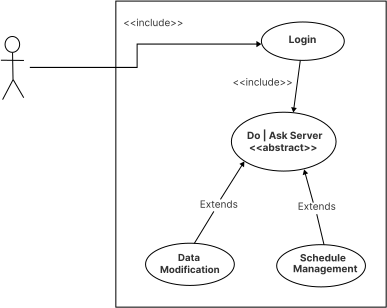
\includegraphics[width=\textwidth]{images/doctorCAS.pdf}
\end{center}
\vspace{-0.85cm}
\begin{center}
	\textit{\textbf{Figure: Doctor Using the App Case Diagram}}
\end{center}

\newpage
\subsubsection*{\textbf{5.2.2 User Interactions (Patients)}}
\addcontentsline{toc}{subsubsection}{5.2.2 User Interactions (Patients)}
Users or patients use the application to find nearby clinics and doctors, check their schedules, and obtain contact details for appointments.

\vspace{0.5cm}
\noindent \textbf{• Use Case Diagram: Patient or User Using the App}
\vspace{0.6cm}
\begin{center}
	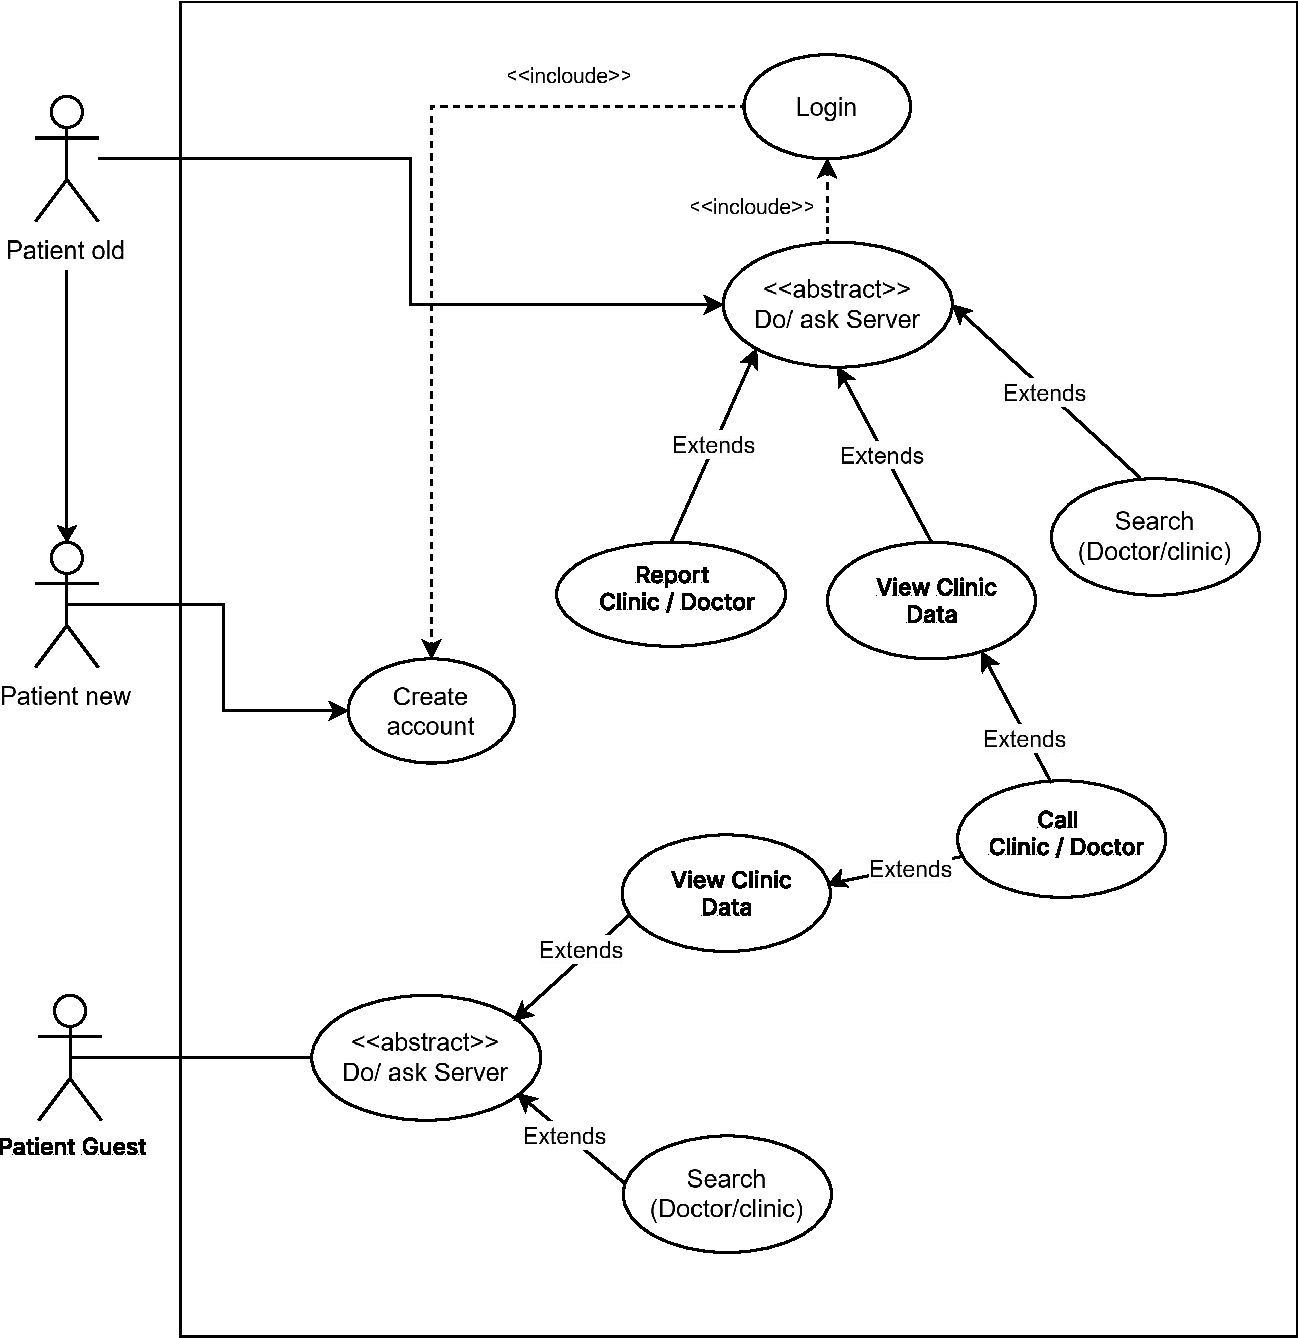
\includegraphics[width=\textwidth]{images/patient@2x.pdf} % Replace "diagram.pdf" with your actual filename
\end{center}
\vspace{-0.35cm}
\begin{center}
	\textit{\textbf{Figure: User Interactions Case Diagram}}
\end{center}
\newpage
\subsubsection*{\textbf{5.2.3 Clinic Interactions}}
\addcontentsline{toc}{subsubsection}{5.2.3 Clinic Interactions}
Clinics are responsible for registering in the application, adding doctors, and managing their clinic details. They must be approved by an admin before becoming active.

\vspace{0.5cm}
\noindent \textbf{• Use Case Diagram: Clinic Using the App}
\vspace{0.6cm}
\begin{center}
	\includegraphics[width=\textwidth]{images/clinicCAS.pdf} % Replace "diagram.pdf" with your actual filename
\end{center}
\vspace{-0.35cm}
\begin{center}
	\textit{\textbf{Figure: Clinic Using the App Case Diagram}}
\end{center}

\newpage
\subsubsection*{\textbf{5.2.4 Admin Interactions}}
\addcontentsline{toc}{subsubsection}{5.2.4 Admin Interactions}
Admins ensure the integrity of the platform by reviewing clinic registration requests and either accepting or rejecting them. They also monitor system performance and maintain security.

\vspace{0.5cm}
\noindent \textbf{• Use Case Diagram: Admin Using the App}
\vspace{0.6cm}
\begin{center}
	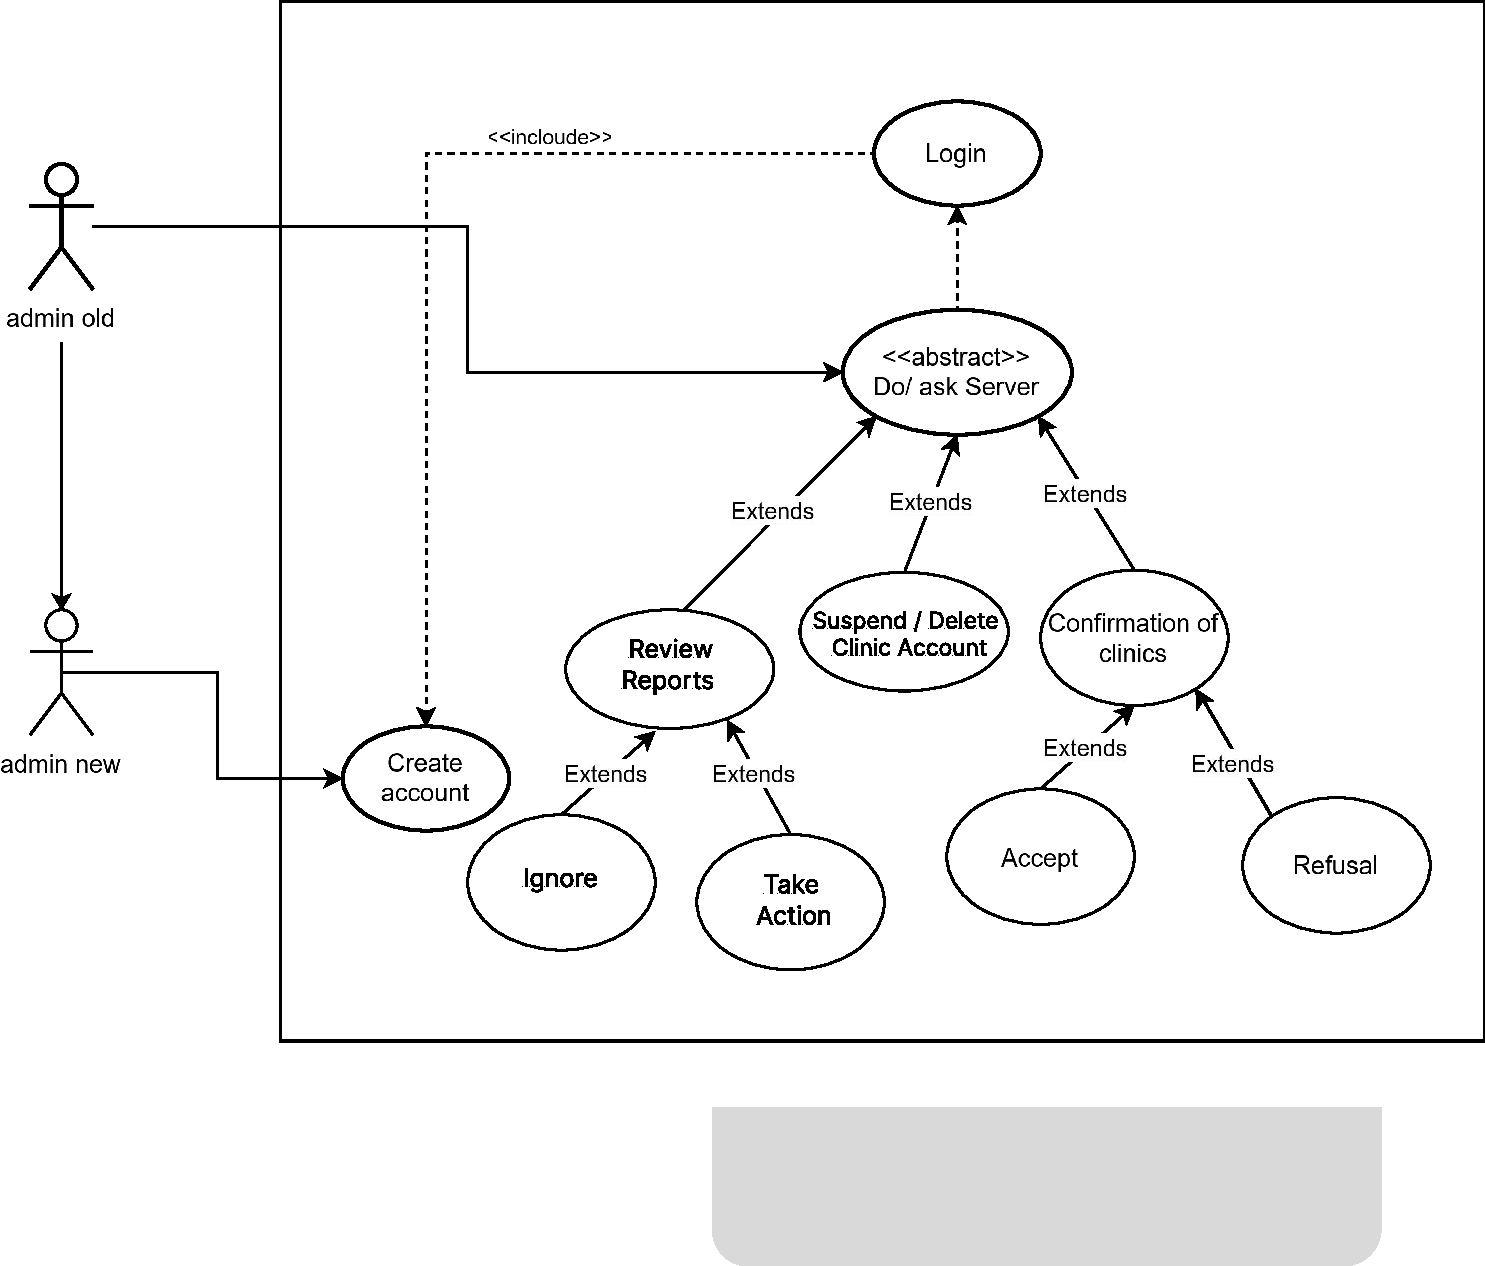
\includegraphics[width=\textwidth]{images/adminCAs@2x.pdf} % Replace "diagram.pdf" with your actual filename
\end{center}
\vspace{-0.35cm}
\begin{center}
	\textit{\textbf{Figure: Admin Using the App Case Diagram}}
\end{center}

\newpage
\section*{\textbf{6 Conclusion}}
\addcontentsline{toc}{section}{6 Conclusion}

\noindent This section has provided a detailed overview of \textbf{Use Case Diagrams} and their role in defining user interactions within the \textbf{Hospital Finder Mobile Application}.\vspace{0.5cm}

\noindent By mapping out different functionalities for doctors, users, clinics, and admins, these diagrams offer a structured approach to understanding the system's behavior.\vspace{0.5cm}

\noindent The next steps involve designing the app structure and implementing the system based on these well-defined interactions.\vspace{0.5cm}

\noindent In the next chapter, we will dive deeper into the app and its conception through additional diagrams, further refining the system's design and architecture.














\newpage

\chapter{\textbf{Application's Conception}}
\rule{\linewidth}{1.5pt}


\section*{\textbf{1 Introduction}}
\addcontentsline{toc}{section}{1 Introduction}

\noindent In this chapter, we present the design phase of our mobile application \textit{Hospital Finder}. Following the analysis and specification of requirements, this stage is essential to define the structural and behavioral aspects of the application.

\noindent The design phase translates the identified functionalities into technical diagrams that guide implementation. These include use case diagrams, class diagrams, and sequence diagrams. Each diagram offers a different perspective, illustrating how components interact and how the system is structured internally.

\subsection*{1.1 Use Case Actors Overview}
\addcontentsline{toc}{subsection}{1.1 Use Case Actors Overview}

\noindent The application involves multiple actors such as:

\begin{itemize}
	\item \textbf{User}: the main end-user searching for hospitals or clinics.
	\item \textbf{Clinic}: responsible for managing their own clinic profile and associated doctors.
	\item \textbf{Admin}: oversees the system and manages reported data or misuse.
	\item \textbf{Doctor}: while present in the system, the doctor does not interact directly with the application and is managed entirely by the clinic.
\end{itemize}
\newpage
\noindent We will observe their interactions more thoroughly in the diagrams presented in the following sections.

\noindent \textbf{A summarized view of the main actors is illustrated in the diagram below :}

\vspace*{0.6cm}
\begin{center}
	\includegraphics[width=0.7\textwidth]{images/AppCycle.pdf}
\end{center}
\vspace{0.1cm}
\begin{center}
	\textit{\textbf{Figure: Application Cycle between App actors .}}
\end{center}
\vspace{0.5cm}

\section*{2 Detailed Design}
\addcontentsline{toc}{section}{2 Detailed Design}

This section presents the core structural design of the \textit{Hospital Finder} application. After analyzing the system’s requirements and actors, we now focus on how these elements are implemented internally.

\noindent The detailed design phase provides a clear \textbf{technical blueprint} by describing the key components, their responsibilities, and how they interact. This allows for a smooth transition from the functional analysis to the actual development.

\noindent \textbf{UML} (Unified Modeling Language) offers various diagrams to describe a software system from different perspectives. These diagrams are generally grouped into two main categories:


\begin{itemize}
	\item \textbf{Structural diagrams} - describe the static aspects of the system, such as classes and their relationships.
	\item \textbf{Behavioral diagrams} - illustrate the dynamic behavior of the system, such as interactions and workflows between components.
\end{itemize}

\begin{center}
	\vspace{1.5cm}
	\hspace{1cm}
	\includegraphics[width=14cm]{images/diagramType.pdf}

\end{center}
\begin{center}
	\textit{\textbf{Figure: Classification of UML diagrams (structure vs behavior).}}
\end{center}
\vspace{0.5cm}
\noindent In Chapter 2, we presented a \textbf{Use Case Diagram}, which belongs to the behavioral category. In this chapter, we will explore two additional diagrams:
\begin{itemize}
	\item The \textbf{Class Diagram}, selected from the structural diagrams.
	\item The \textbf{Sequence Diagram}, selected from the behavioral diagrams.
\end{itemize}

\noindent These diagrams allow us to model both the architecture and the interactions in our application in a clear and structured manner. We begin with the class diagram in the next section.

\subsection*{2.1 Class Diagram}
\addcontentsline{toc}{subsection}{2.1 Class Diagram}

A class diagram plays a key role in the object-oriented design of software systems. In this section, we will define what a class diagram is, explain its importance in the development process, and finally present the class diagram of our \textit{Hospital Finder} application.

\subsubsection*{2.1.1 What is a Class Diagram ?}
\addcontentsline{toc}{subsubsection}{2.1.1 What is a Class Diagram ?}
\vspace{0.1cm}

A \textbf{class diagram} is a static structural diagram that describes the types of objects in the system and the various kinds of \textbf{relationships} that exist among them. It shows the system's \textbf{classes}, their \textbf{attributes}, \textbf{methods}, and the \textbf{associations} between objects. It is one of the most commonly used diagrams in \textbf{UML} (Unified Modeling Language) and serves as a \textbf{blueprint} for the \textbf{implementation phase}.

\noindent Each class is represented as a rectangle divided into compartments. The top compartment shows the \textbf{class name}, the middle one lists the \textbf{attributes}, and the bottom lists the \textbf{operations} or \textbf{methods}.


\subsubsection*{2.1.2 Why Use a Class Diagram ?}
\addcontentsline{toc}{subsubsection}{2.1.2 Why Use a Class Diagram ?}
\vspace{0.1cm}


The \textbf{class diagram} is essential in the software development lifecycle for the following reasons:

\begin{itemize}
	\item It provides a visual overview of the system \textbf{structure}.
	\item It helps developers understand how \textbf{data} is organized and managed.
	\item It facilitates the identification of responsibilities and roles of each class.
	\item It reflects both the logical architecture and the design of the application's \textbf{database}.
	\item It helps in detecting potential \textbf{design flaws} early in the development process.
\end{itemize}

\noindent In the context of our project, the \textbf{class diagram} acts as a bridge between the \textbf{actors} (users, clinics, doctors, and admins) and the data handled internally. It helps clarify how the \textbf{components} of the system interact with one another and ensures a consistent and maintainable code structure.


\subsubsection*{2.1.3 Class Diagram of the Application}
\addcontentsline{toc}{subsubsection}{2.1.3 Class Diagram of the Application}
\vspace{0.1cm}


The class diagram of the \textit{Hospital Finder} application was developed based on the functional and non-functional requirements outlined during the analysis phase. It models the following key classes:
\begin{itemize}

	\item \textbf{users}: Stores core information for every system user.
	      \begin{itemize}
		      \item \texttt{id}: Primary key.
		      \item \texttt{google\_id}: Used for Google login.
		      \item \texttt{name}, \texttt{email}: Basic user details.
		      \item \texttt{user\_notify\_status}: Boolean for notifications.
		      \item \texttt{fcm\_token}: Firebase push notifications.
		      \item \texttt{user\_role}: Role type (small integer).
		      \item \texttt{profile\_image}: User profile picture.
	      \end{itemize}

	\item \textbf{role}: Defines all possible user roles.
	      \begin{itemize}
		      \item \texttt{id}: Primary key.
		      \item \texttt{role\_name}: Name of the role.
	      \end{itemize}

	\item \textbf{roles\_user}: Connects users and roles (many-to-many).
	      \begin{itemize}
		      \item \texttt{id}: Primary key.
		      \item \texttt{user\_id}, \texttt{role\_id}: User and role references.
	      \end{itemize}

	\item \textbf{specialties}: Medical specialties.
	      \begin{itemize}
		      \item \texttt{id}: Primary key.
		      \item \texttt{name}, \texttt{name\_fr}: Names (default and French).
		      \item \texttt{specialy\_img}: Optional image.
	      \end{itemize}

	\item \textbf{municipalities}: Cities or regions.
	      \begin{itemize}
		      \item \texttt{id}: Primary key.
		      \item \texttt{name}, \texttt{name\_fr}: Names (default and French).
	      \end{itemize}

	\item \textbf{clinic\_schedules}: Clinic working hours.
	      \begin{itemize}
		      \item \texttt{id}: Primary key.
		      \item \texttt{clinic\_id}: Linked clinic.
		      \item \texttt{day}, \texttt{opening\_time}, \texttt{closing\_time}: Work schedule.
	      \end{itemize}

	\item \textbf{Clinics}: Registered health facilities.
	      \begin{itemize}
		      \item \texttt{id}: Primary key.
		      \item \texttt{user\_id}: Linked user.
		      \item \texttt{municipalities\_id}: Linked municipality.
		      \item \texttt{name}, \texttt{type}: Name and type (clinic/hospital).
		      \item \texttt{address}, \texttt{Statue}: Location and status.
	      \end{itemize}

	\item \textbf{doctor}: Medical professional profiles.
	      \begin{itemize}
		      \item \texttt{id}: Primary key.
		      \item \texttt{user\_id}, \texttt{clinic\_id}, \texttt{specialties\_id}: Linked user, clinic, specialty.
		      \item \texttt{name}, \texttt{Presence}: Name and availability.
	      \end{itemize}

	\item \textbf{Doctor\_schedules}: Doctor working hours.
	      \begin{itemize}
		      \item \texttt{id}: Primary key.
		      \item \texttt{clinic\_id}: Linked doctor.
		      \item \texttt{day}, \texttt{opening\_time}, \texttt{closing\_time}: Schedule.
	      \end{itemize}

	\item \textbf{notifications}: System notifications.
	      \begin{itemize}
		      \item \texttt{id}: Primary key.
		      \item \texttt{title}, \texttt{content}: Notification message.
		      \item \texttt{is\_read}: Read status.
		      \item \texttt{user\_id}: Recipient.
	      \end{itemize}

	\item \textbf{reports}: User reports against others.
	      \begin{itemize}
		      \item \texttt{id}: Primary key.
		      \item \texttt{reporter\_id}, \texttt{reported\_id}: Reporter and reported users.
	      \end{itemize}

\end{itemize}

\vspace{4cm}
\begin{center}
	\textbf{ The class diagram is shown below : }
\end{center}
\begin{center}
	\hspace*{-1cm}\includegraphics[width=1.1\textwidth]{images/dbclass.pdf}
\end{center}
\vspace{0.5cm}
\begin{center}
	\textit{\textbf{Figure: Class diagram of the Hospital Finder application.}}

\end{center}
\vspace{0.5cm}
\subsection*{2.2 Sequence Diagrams}
\addcontentsline{toc}{subsection}{2.2 Sequence Diagrams}
\vspace{-0.3cm}
\rule{7.2cm}{1.2pt}
\vspace{-0.3cm}

\subsubsection*{2.2.1 Definition}
\addcontentsline{toc}{subsubsection}{2.2.1 Definition}
\vspace{0.1cm}

Sequence diagrams are a type of UML behavioral diagram that show how objects or components in a system interact with each other over time. They describe the flow of messages and the order of operations between actors and system parts in specific scenarios.

Each sequence diagram illustrates how different entities collaborate in a particular process, using lifelines, messages, and activation bars to convey their roles and responsibilities.

\subsubsection*{2.2.2 Purpose and Importance}
\addcontentsline{toc}{subsubsection}{2.2.2 Purpose and Importance}
\vspace{0.1cm}


\textbf{Sequence diagrams} are essential for modeling \textbf{dynamic behavior} in a system. They help developers understand the exact \textbf{flow of operations}, communication between objects, and timing of events.

In our case, these diagrams allow us to:
\begin{itemize}
	\item Clearly visualize \textbf{interactions} between the application interface, users (like admin), and the backend (\textbf{database}).
	\item Ensure that the designed processes are logically consistent and complete.
\end{itemize}


\subsubsection*{2.2.3 Application Sequence Diagrams}
\addcontentsline{toc}{subsubsection}{2.2.3 Application Sequence Diagrams}
\vspace{0.1cm}

Below, we present a set of sequence diagrams that demonstrate different operations carried out by the admin user. Each diagram focuses on a specific use case and models the message flow involved.

\newpage

\begin{minipage}{\textwidth}
	\noindent\underline{\textbf{• Searching for a Clinic or Doctor:}}
	This diagram models the process in which the user searches for a clinic or doctor.

	\vspace{0.9cm}

	\begin{sequencediagram}
		% Participants with increased spacing
		\newinst[1]{U}{User}
		\newinst[4]{S}{App Interface}
		\newinst[4]{DB}{Database}

		% Login and Initial Search
		\begin{call}{U}{Login(username, password)}{S}{}
			\begin{call}{S}{Validate Credentials}{DB}{Result}
			\end{call}
			\begin{sdblock}{alt}{Are credentials valid?}
				\begin{sdblock}{option}{Yes}
					\mess{S}{Login Success}{U}
				\end{sdblock}
				\begin{sdblock}{option}{No}
					\mess{S}{Login Failed or Search as Guest}{U}
				\end{sdblock}
			\end{sdblock}
		\end{call}

		\postlevel
		\vspace{0.5cm}
		\prelevel

		% Search Loop
		\begin{sdblock}{loop}{Until valid clinic/doctor found}
			\begin{call}{U}{Enter Clinic/Doctor Name}{S}{}
			\end{call}

			\begin{call}{S}{Search Records}{DB}{Search Results}
			\end{call}

			\begin{sdblock}{alt}{Found?}
				\begin{sdblock}{Yes}{}
					\begin{call}{S}{Display Results}{U}{}
					\end{call}
				\end{sdblock}

				\begin{sdblock}{No}{}
					\begin{call}{S}{Show "Not Found" Error}{U}{}
					\end{call}
					\begin{call}{U}{Retry Search}{S}{}
					\end{call}
				\end{sdblock}
			\end{sdblock}
		\end{sdblock}

		\begin{call}{S}{Display Final Results}{U}{}
		\end{call}
	\end{sequencediagram}


\end{minipage}

\noindent\underline{\textbf{• Clinic Registering In The Application :}}
This sequence diagram illustrates the process by which a clinic registers on the app. The clinic submits information through the app, which is then stored in the database. Admin verifies the submission and either approves or rejects the registration.

\vspace{1cm}

\begin{sequencediagram}
	% Participants with increased spacing
	\newinst[0]{C}{Clinic/Doctor}
	\newinst[1.5]{A}{App Interface}
	\newinst[1.5]{DB}{Database}
	\newinst[2]{Ad}{Admin}

	% Registration Flow
	\begin{call}{C}{Submit Information}{A}{}
		\begin{call}{A}{Store Information}{DB}{Storage Result}
		\end{call}
		\mess{A}{Submission Received}{C}
	\end{call}

	% Admin Verification
	\postlevel
	\vspace{1cm}
	\prelevel

	\begin{call}{DB}{Check Pending Requests}{Ad}{Registration Data}
	\end{call}

	\begin{sdblock}{Alternative}{Admin Decision}
		\begin{sdblock}{Acceptance}{}
			\begin{call}{DB}{Approve Account}{Ad}{}
			\end{call}
			\mess{Ad}{Send Approval}{A}
			\mess{A}{Account Approved}{C}
		\end{sdblock}

		\begin{sdblock}{Refusal}{}
			\begin{call}{DB}{Reject Application}{Ad}{}
			\end{call}
			\mess{Ad}{Send Rejection}{A}
			\mess{A}{Account Rejected}{C}
		\end{sdblock}
	\end{sdblock}

	% Login After Approval
	\postlevel
	\vspace{1cm}
	\prelevel

	\begin{sdblock}{Optional}{If Approved}
		\begin{call}{C}{Login}{A}{}
			\begin{call}{A}{Verify Credentials}{DB}{}
			\end{call}
			\begin{call}{A}{Grant Access}{C}{}
			\end{call}
		\end{call}
	\end{sdblock}
\end{sequencediagram}

\noindent\underline{\textbf{• Clinic Managing Doctor Accounts (Add, Delete, Suspend) :}}
This sequence diagram illustrates how a clinic directly manages doctor accounts—adding, deleting, or suspending—through the application interface. All operations interact with the database without any admin involvement.

\vspace{1cm}

\begin{sequencediagram}
	% Participants
	\newinst[0]{C}{Clinic}
	\newinst[4]{A}{App Interface}
	\newinst[4]{DB}{Database}

	% Adding a Doctor
	\begin{sdblock}{Add Doctor}{}
		\begin{call}{C}{Enter Doctor Details}{A}{}
			\begin{call}{A}{Store Doctor Info}{DB}{Success}
			\end{call}
			\mess{A}{Doctor Account Created}{C}
		\end{call}
	\end{sdblock}

	% Deleting a Doctor
	\postlevel
	\vspace{0.8cm}
	\prelevel
	\begin{sdblock}{Delete Doctor}{}
		\begin{call}{C}{Select Doctor to Delete}{A}{}
			\begin{call}{A}{Delete Doctor Record}{DB}{Success}
			\end{call}
			\mess{A}{Doctor Account Deleted}{C}
		\end{call}
	\end{sdblock}

	% Suspending a Doctor
	\postlevel
	\vspace{0.8cm}
	\prelevel
	\begin{sdblock}{Suspend Doctor}{}
		\begin{call}{C}{Choose Doctor to Suspend}{A}{}
			\begin{call}{A}{Update Status to Suspended}{DB}{Success}
			\end{call}
			\mess{A}{Doctor Account Suspended}{C}
		\end{call}
	\end{sdblock}

\end{sequencediagram}

\newpage
\noindent\underline{\textbf{• Admin Managing Clinics Requests:}}
This sequence diagram models the process by which the admin handles clinic registration requests. The admin reviews the applications, makes a decision, and updates the database accordingly.

\vspace*{0.9cm}


\begin{sequencediagram}
	% Participants with increased spacing
	\newinst[0]{Ad}{Admin}
	\newinst[4]{A}{App Interface}
	\newinst[4]{DB}{Database}

	% Access Requests List
	\begin{call}{Ad}{Access Request List}{A}{}
		\begin{call}{A}{Fetch Pending Requests}{DB}{Requests Data}
		\end{call}
	\end{call}

	% Review Process
	\postlevel
	\vspace{0.5cm}
	\prelevel

	\begin{sdblock}{Loop}{For each application}
		\begin{call}{Ad}{Select Application}{A}{}
		\end{call}

		\begin{call}{Ad}{Review Details}{A}{}
			\begin{call}{A}{Get Full Application}{DB}{Complete Data}
			\end{call}
		\end{call}

		\begin{sdblock}{Alternative}{Decision}
			\begin{sdblock}{Acceptance}{}
				\begin{call}{Ad}{Confirm Approval}{A}{}
					\begin{call}{A}{Update Status}{DB}{Approved}
					\end{call}
				\end{call}
				\mess{DB}{Approval Notification}{Ad}  % To notify clinic
			\end{sdblock}

			\begin{sdblock}{Refusal}{}
				\begin{call}{Ad}{Confirm Rejection}{A}{}
					\begin{call}{A}{Update Status}{DB}{Rejected}
					\end{call}
				\end{call}
				\mess{DB}{Rejection Notification}{Ad}  % To notify clinic
			\end{sdblock}
		\end{sdblock}
	\end{sdblock}

	% Completion
	\postlevel
	\vspace{0.5cm}
	\prelevel
	\mess{A}{Processing Complete}{Ad}
\end{sequencediagram}

\newpage

\noindent\underline{\textbf{• User Report Activity:}}
This sequence diagram models the process when a user submits a report. After submission, the admin reviews the report and takes action, which may result in a notification being sent to the user.

\vspace*{1cm}

\begin{sequencediagram}
	% Participants with increased spacing
	\newinst[0]{U}{User}
	\newinst[2.4]{A}{App Interface}
	\newinst[2.1]{DB}{Database}
	\newinst[2.1]{Ad}{Admin}

	% Reporting Flow
	\begin{call}{U}{Submit Report}{A}{}
		\begin{call}{A}{Store Report}{DB}{Confirmation}
		\end{call}
		\mess{A}{Report Submitted notification}{U}
	\end{call}

	% Admin Review Process
	\postlevel
	\vspace{0.5cm}
	\prelevel

	\begin{call}{Ad}{Check New Reports}{DB}{Report Data}
	\end{call}

	\begin{sdblock}{Alternative}{Report Validation}
		\begin{sdblock}{Valid Report}{}
			\begin{call}{Ad}{Restrict Clinic}{DB}{}
				\begin{call}{DB}{Update Status}{DB}{Restricted}
				\end{call}
			\end{call}
			\mess{Ad}{Notify Action Taken}{A}
		\end{sdblock}

		\begin{sdblock}{False Report}{}
			\begin{call}{Ad}{Mark as False}{DB}{}
			\end{call}
			\mess{Ad}{Ignore Report}{A}
		\end{sdblock}
	\end{sdblock}

	% Notification
	\postlevel
	\vspace{0.5cm}
	\prelevel
	\mess{DB}{Status Updated}{A}
\end{sequencediagram}


\newpage
\section*{3 Conclusion}
\addcontentsline{toc}{section}{3 Conclusion}

\vspace{1em}

\noindent
The design phase of our \textit{Hospital Finder} mobile application has been carefully structured to ensure clarity, consistency, and extensibility. Throughout this chapter, we laid the foundation of the application by modeling its components and interactions using essential UML diagrams.
\vspace{1em}

\noindent
We began with the class diagram, which defined the main entities such as users, clinics, doctors, and the admin, along with their relationships. This provided a blueprint for structuring the database and guiding the backend development. Each class was tailored to support the application's functionality, ensuring that both user and system needs are represented.

\vspace{1em}

\noindent
Subsequently, we introduced a series of sequence diagrams to illustrate the dynamic behavior of the system. These diagrams covered key interactions including user registration, clinic requests, login, searching, and admin management operations. Particular focus was placed on administrator features—such as reviewing clinic applications and handling user reports—emphasizing the application's flexibility and administrative control.

\vspace{1em}

\noindent
Each interaction was modeled to ensure that data flows seamlessly through the app interface and is consistently stored or retrieved from the database. The logical flow within these diagrams also helps in pinpointing edge cases, user roles, and error-handling scenarios.

\vspace{1em}

\noindent
In summary, this conception phase has transformed abstract requirements into detailed structural and behavioral models. These models not only support the system’s current requirements but also anticipate future enhancements. The groundwork laid here will facilitate a smoother transition to the implementation phase, ensuring that development is aligned with the overall system design.















\newpage

\chapter{The Implementation of our App}
\section*{1 Introduction}
\addcontentsline{toc}{section}{1 Introduction}
This chapter is dedicated to the practical realization of our mobile application. It provides a detailed overview of the technical environment in which the project was developed and tested, including both hardware and software components.\vspace{0.5cm}

\noindent We will begin by presenting the development and testing equipment used, followed by the tools and technologies adopted throughout the implementation process. In addition, we will present the application's key interfaces and explain how they interact.\vspace{0.5cm}

\noindent Finally, this chapter will showcase selected code snippets and logic responsible for handling certain events and functionalities in the application — offering a clear view of the internal mechanisms that drive the user experience.


\section*{2 Work Environment}
\addcontentsline{toc}{section}{2 Work Environment}
\vspace{-0.5cm}
\rule{0.45\linewidth}{1pt} \\[-1.2cm]
\subsection*{2.1 Hardware Environment}
\addcontentsline{toc}{subsection}{2.1 Hardware Environment}
For development and testing, the following hardware was used:

\begin{itemize}
	\item \textbf{Development Machines:}
	      \begin{itemize}
		      \item \textbf{HP EliteBook 840 G4} – Intel Core i5-7200U, 16GB DDR4 RAM (2444MHz), 256GB SSD.
		      \item \textbf{Dell Laptop 1} – Intel Core i5 9th Gen, 16GB RAM.
		      \item \textbf{Dell Laptop 2} – Intel Core i5 6th Gen, 16GB RAM.
	      \end{itemize}

	\item \textbf{Test Devices:}
	      \begin{itemize}
		      \item Samsung Galaxy S21
		      \item Samsung Galaxy S21 FE
		      \item Redmi Note 8 Pro
	      \end{itemize}
\end{itemize}

\subsection*{2.2 Software Environment}
\addcontentsline{toc}{subsection}{2.2 Software Environment}
\vspace{-0.3cm}
\rule{0.40\linewidth}{0.5pt} \\[-1.2cm]
\subsubsection*{2.2.1 Technologies Used}
\addcontentsline{toc}{subsubsection}{2.2.1 Technologies Used}
It presents the main technologies adopted, such as the programming language, development platform, and the chosen database management .

\begin{itemize}
	\item \textbf{Programming Language:} The most vital and indispensable tool in our project is \textbf{Dart}, used through the \textbf{Flutter} framework. Flutter enables us to develop a cross-platform mobile application (Android and iOS) from a single codebase, significantly accelerating development and ensuring a consistent user experience. Below is a flowchart to illustrate how Flutter operates:
	      \vspace{0.5cm}
	      \begin{center}
		      \includegraphics[width=\linewidth]{images/FlutterDiagram@2x.pdf}
		      \textit{\textbf{Figure: Flutter Architecture Flowchart}}
	      \end{center}


	\item \textbf{Development Environments:} We primarily used \textbf{Visual Studio Code} and \textbf{Android Studio} as our code editors and development environments, which are widely recognized and powerful for mobile app development.

	\item \textbf{Backend:} We chose the \textbf{Laravel} PHP framework for creating the backend API. It provided us with a clear MVC structure, enhanced security, and easy management of routes and controllers.

	\item \textbf{Database:} The application uses a \textbf{MySQL} database, which we designed and hosted on a \textbf{Hostinger} server. The backend files were also deployed on this server to handle API communication with the mobile app.

	\item \textbf{Firebase:} Integrated for backend services, particularly \textbf{authentication}. We used \textbf{Google Console} to enable patients to log in using their Google accounts.

	\item \textbf{Testing Tools:} We used \textbf{Postman} to test various API requests and endpoints before integrating them into the mobile app.

	\item \textbf{Version Control:} Our source code was managed using \textbf{Git} and hosted on \textbf{GitHub}, which facilitated team collaboration and version tracking.

	\item \textbf{Design Tools:} We used \textbf{Figma} to design the user interface of the app and create user flow diagrams. For database modeling and class diagrams, we used \textbf{dbdiagram.io}.

\end{itemize}

\subsection*{2.3 Database Management System}
\addcontentsline{toc}{subsection}{2.3 Database Management System}
\rule{0.40\linewidth}{0.5pt} \\[-1.0cm]
\subsubsection*{• 2.3.1 Overview and Tools}
\addcontentsline{toc}{subsubsection}{2.3.1 Overview and Tools}
In this project, special focus was given to designing and implementing the database using Laravel, which provides an efficient system for migrations, models, and seeders. This section describes the workflow, tools, and structure adopted for managing data throughout the application.

\noindent The database schema was initially designed using \textbf{dbdiagram.io}, a web-based tool for visualizing tables, fields, and relationships. This served as a blueprint, ensuring a well-structured relational database before implementation.

\noindent Throughout development, \textbf{phpMyAdmin} was used to manage and inspect the MySQL database, complementing Laravel’s command-line tools for data verification and query testing.

\vspace{0.5cm}

\subsubsection*{• 2.3.2 Implementation with Laravel}
\addcontentsline{toc}{subsubsection}{2.3.2 Implementation with Laravel}

The schema was implemented using Laravel’s \textbf{migration system}, with each table defined in separate migration files, specifying columns, data types, keys, and constraints. Laravel’s migrations provide version control, simplifying maintenance and scaling.

\noindent \textbf{Eloquent models} were created for each table, acting as an abstraction layer to handle operations like insertion, updates, deletion, and retrieval. These models also define interrelations (e.g., \texttt{hasMany}, \texttt{belongsTo}), reflecting the relational schema.

\noindent \textbf{Seeders} were used to populate the database with essential data, useful during development, testing, or first-time deployments.

\vspace{0.5cm}

\subsubsection*{• 2.3.3 Authentication and Access Control}
\addcontentsline{toc}{subsubsection}{2.3.3 Authentication and Access Control}

While backend authentication is covered in another section, the system enforces strict \textbf{role-based access control} (RBAC). Each user (doctor, clinic, admin, general user) receives an assigned role, and access permissions are enforced accordingly.

\noindent \textbf{Firebase Authentication} (email/password, Google Sign-In) is integrated via the \textbf{Google Cloud Console}. After client-side login (Flutter), a Firebase token is sent to the backend, where Laravel verifies it using the Firebase Admin SDK and issues a Laravel session token with \textbf{Laravel Sanctum}.

\noindent \textbf{Sanctum} securely manages API tokens and sessions. Custom middleware checks the user’s Firebase UID, fetches their role, and enforces permissions, returning a 403 error for unauthorized actions.

\vspace{0.5cm}

\subsubsection*{• 2.3.4 Diagrams and Database Schema}
\addcontentsline{toc}{subsubsection}{2.3.4 Diagrams and Database Schema}

The diagrams below illustrate two key components:
\begin{itemize}
	\item \textbf{MVC Architecture} of our app with models, controllers, and views. Note that the shown models, views, and controllers are only a few examples of the many present in the application. Each use case’s components are consistently represented in the same color, helping to visually group related parts.
	\item \textbf{Laravel Sanctum flow}, demonstrating how tokens are validated before requests reach the database and Hostinger API. The flow includes step indicators:

	      \par \texttt{1.1} – Generate Token On Login
	      \par \texttt{2.1} – Api Request
	      \par \texttt{2.2} – Check of Token is Valid Using Laravel Sanctum Api
	      \par \texttt{2.3} – Reject if not Valid
	      \par \texttt{3.1} – Allow Data Access ( CRED Operation )
	      \par \texttt{3.2} – Response ( OK / Not OK )
	      \par \texttt{3.3} – Display Response
	      \par \texttt{4.1} – Avoid 3rd parties Api from accessing our App api using sanctum

\end{itemize}
\vspace*{0.4cm}
\begin{figure}[H]
	\centering
	\includegraphics[width=1\textwidth]{images/sanctum@2x.pdf}
\end{figure}
\begin{center}
	\vspace*{0.3cm}
	\textit{Figure: Authentication Laravel Sanctum Token Validation Before Database/API Access.}
\end{center}
\vspace*{0.8cm}
\begin{figure}[H]
	\centering
	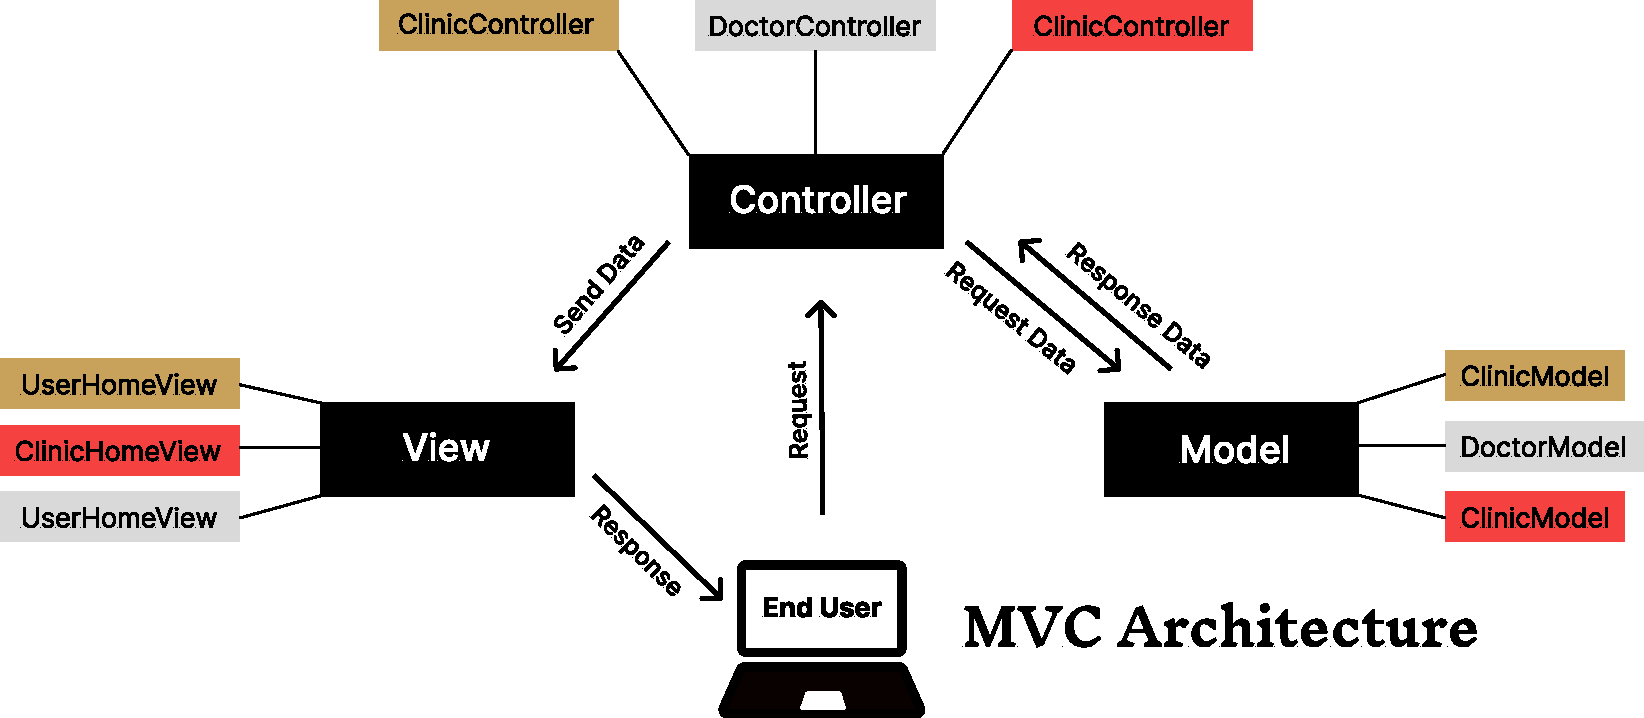
\includegraphics[width=1\textwidth]{images/MVC@2x.pdf}
\end{figure}
\begin{center}
	\vspace*{0.3cm}
	\textit{Figure: Our App MVC Architecture: Model-Controller-View Structure }
\end{center}


\newpage
\noindent For our database tables we show below some of our core tables \textbf{— \texttt{users}, \texttt{clinics}, \texttt{doctors},\texttt{role},\texttt{Schedule} and \texttt{Sanctum Validation Table} — }represent the heart of the system. Their schemas are shown below.
\vspace*{0.5cm}
\begin{figure}[H]
	\centering
	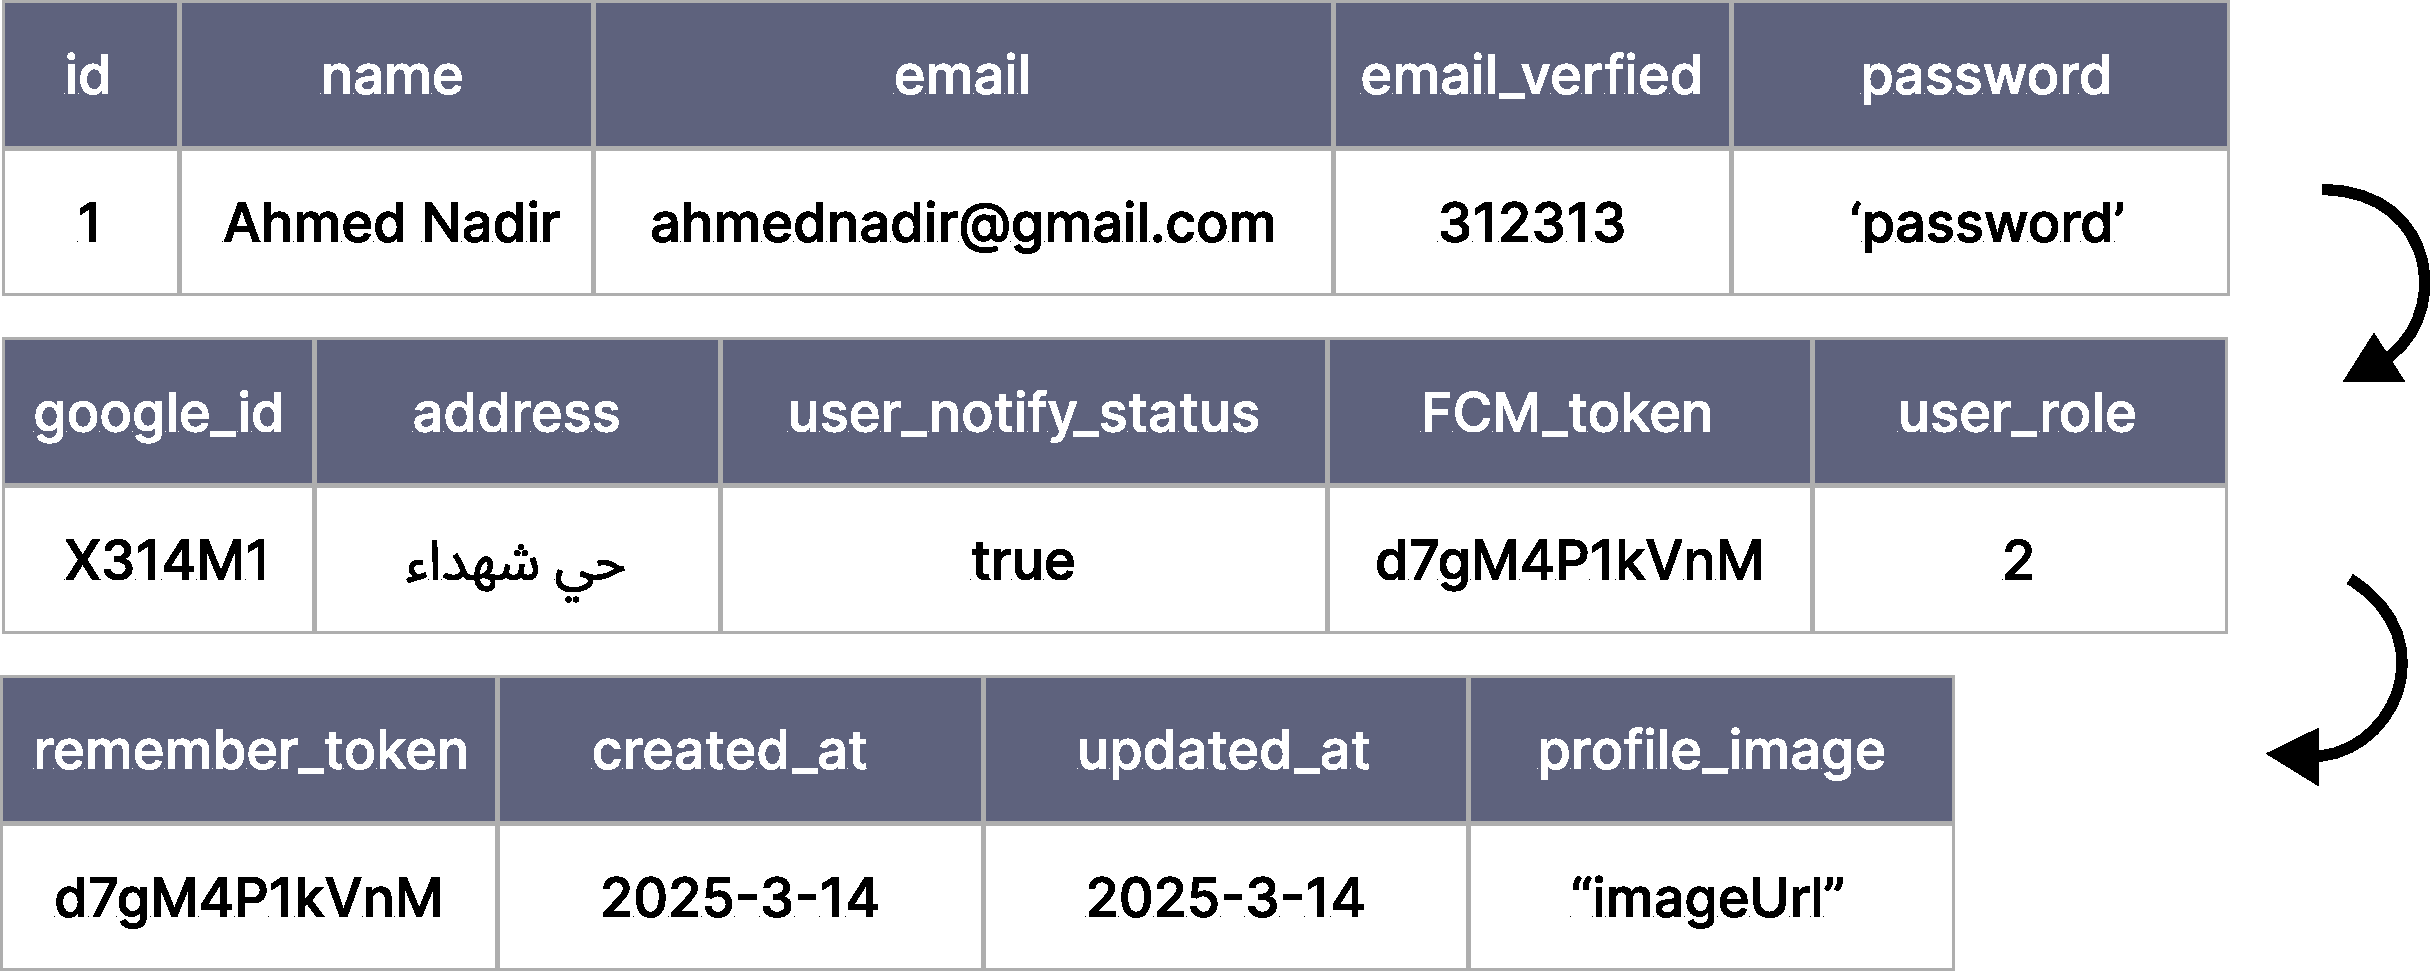
\includegraphics[width=0.9\textwidth]{images/user_table.pdf}
\end{figure}
\begin{center}
	
	\textbf{\textit{Figure: Users Table Schema}}
\end{center}

\begin{figure}[H]
	\centering
	\hspace*{-0.5cm}
	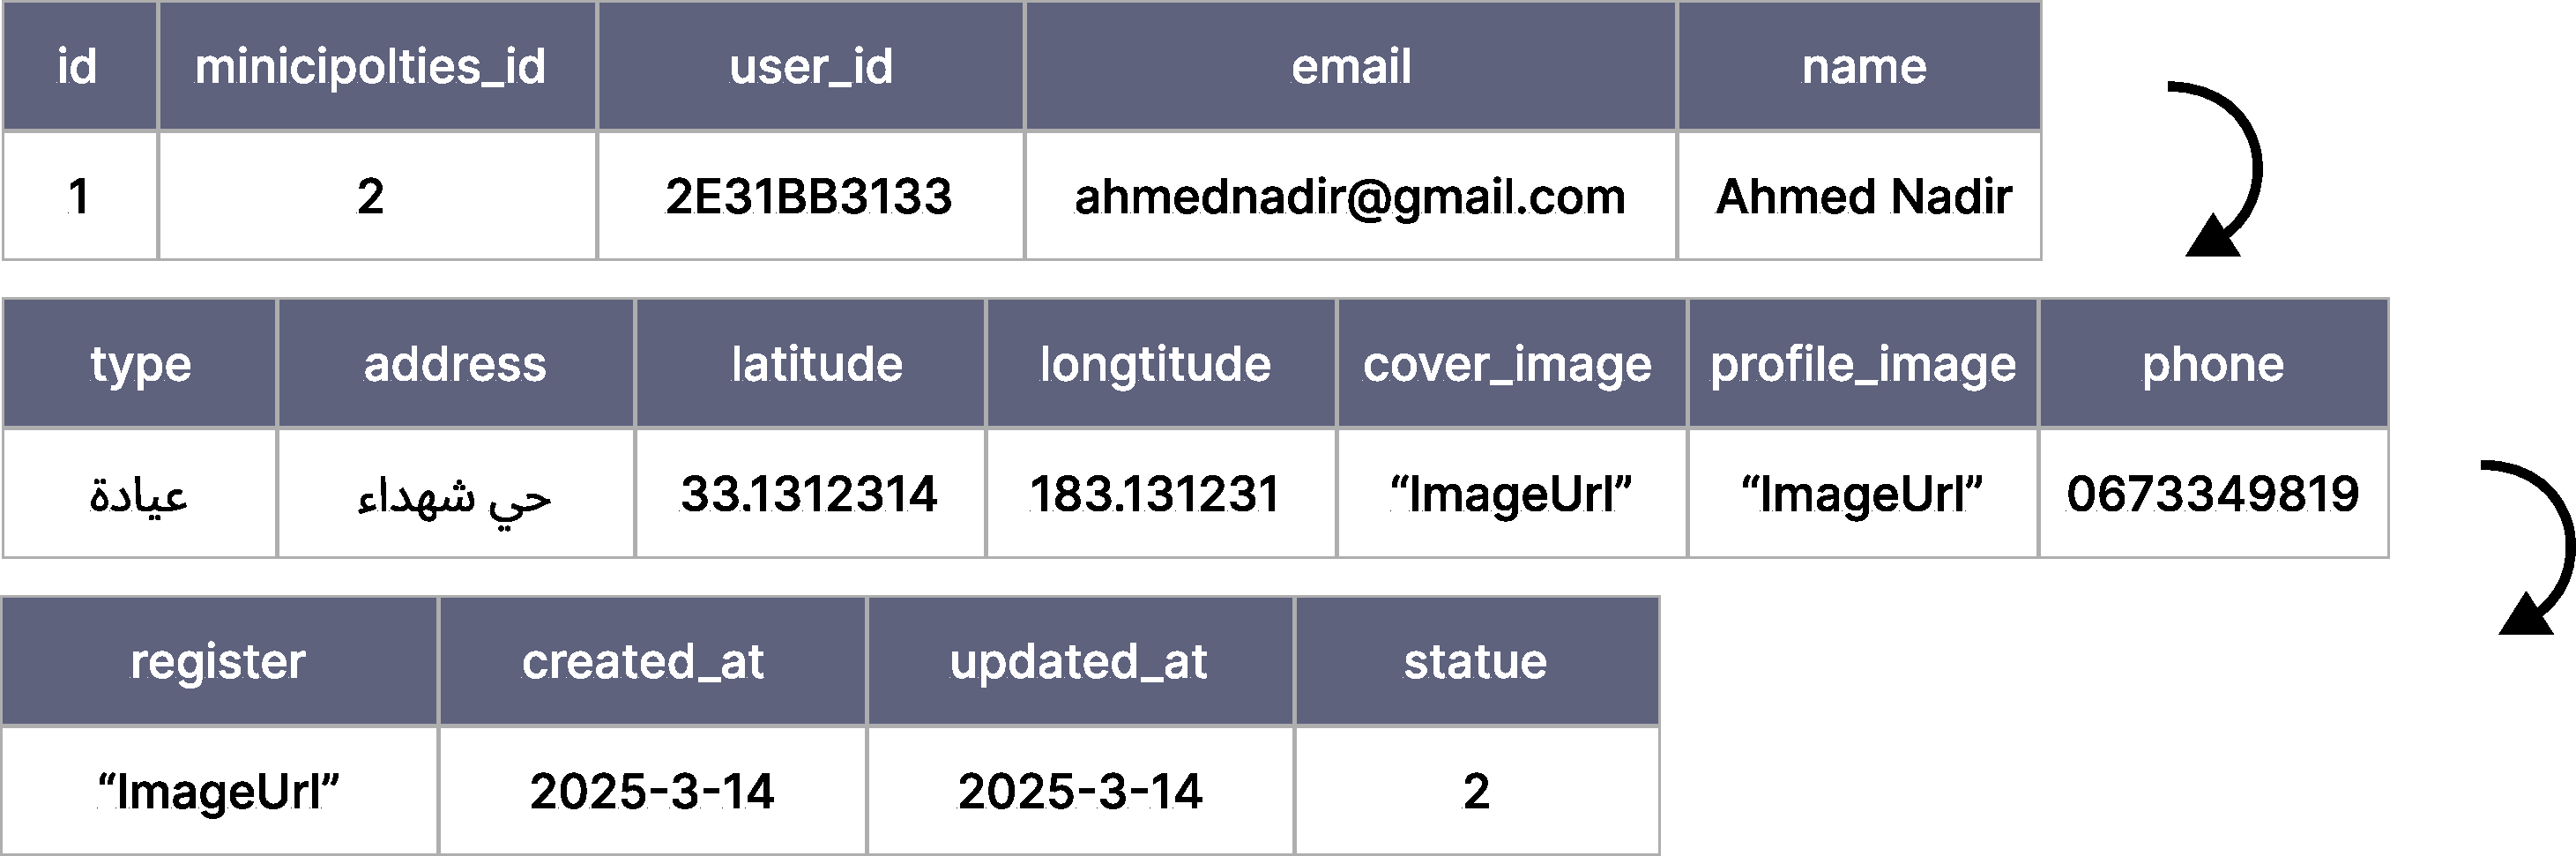
\includegraphics[width=1.1\textwidth]{images/clinic_table@2x.pdf}
\end{figure}
\begin{center}
	\textbf{\textit{Figure: Clinics Table Schema}}
\end{center}


\begin{figure}[H]
	\centering
	\hspace*{-0.7cm}
	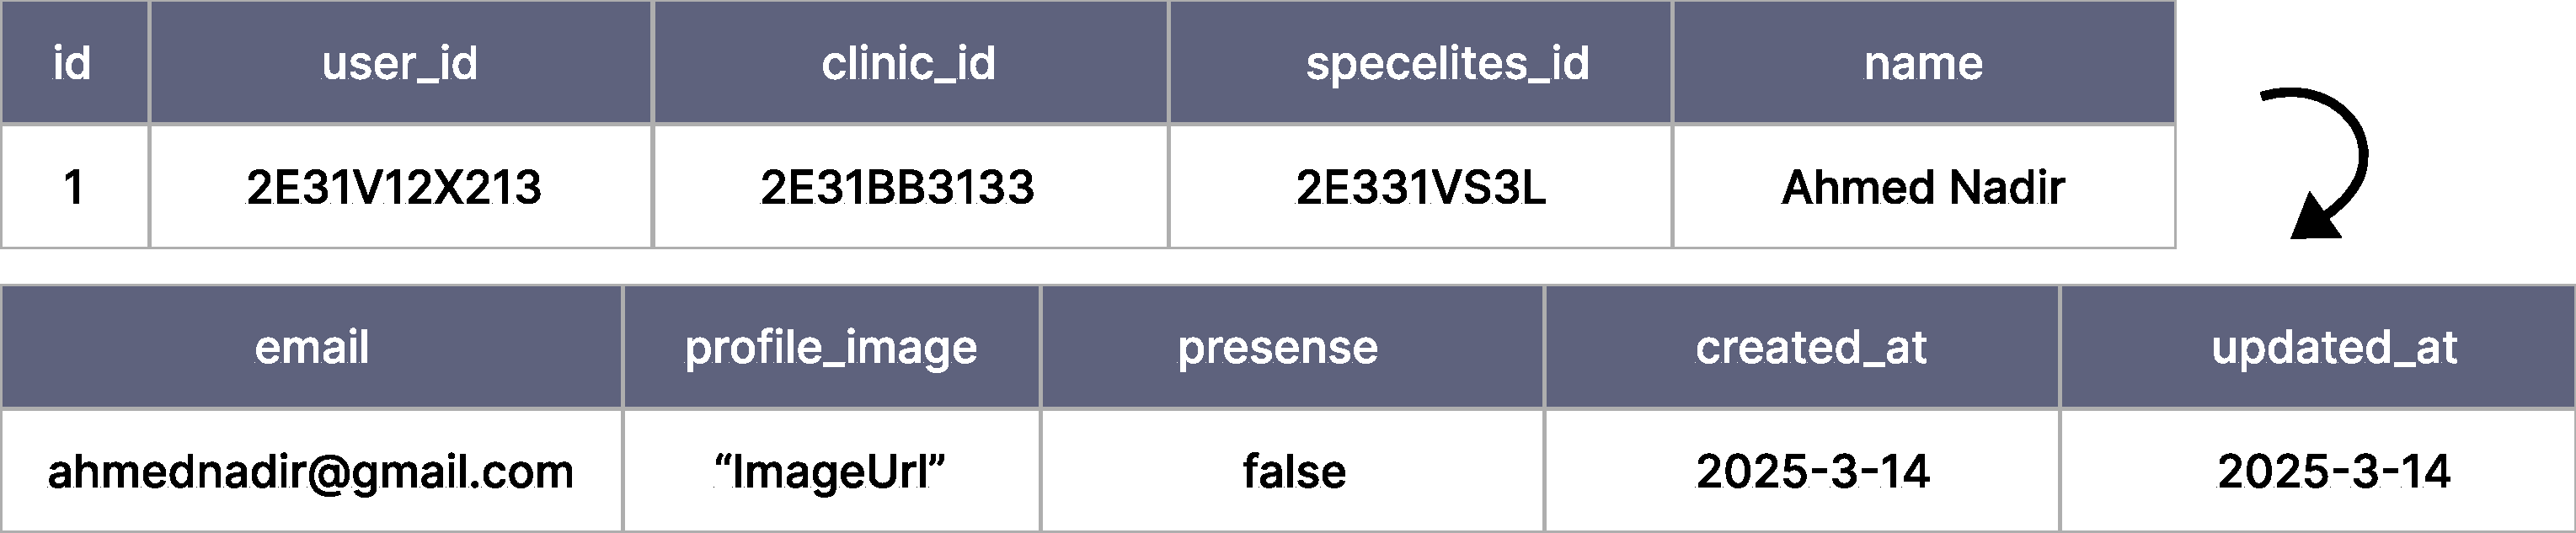
\includegraphics[width=1.1\textwidth]{images/doctor_table@2x.pdf}
\end{figure}
\begin{center}
	\textbf{\textit{Figure: Doctor Table Schema}}
\end{center}

\begin{figure}[H]
	\centering
	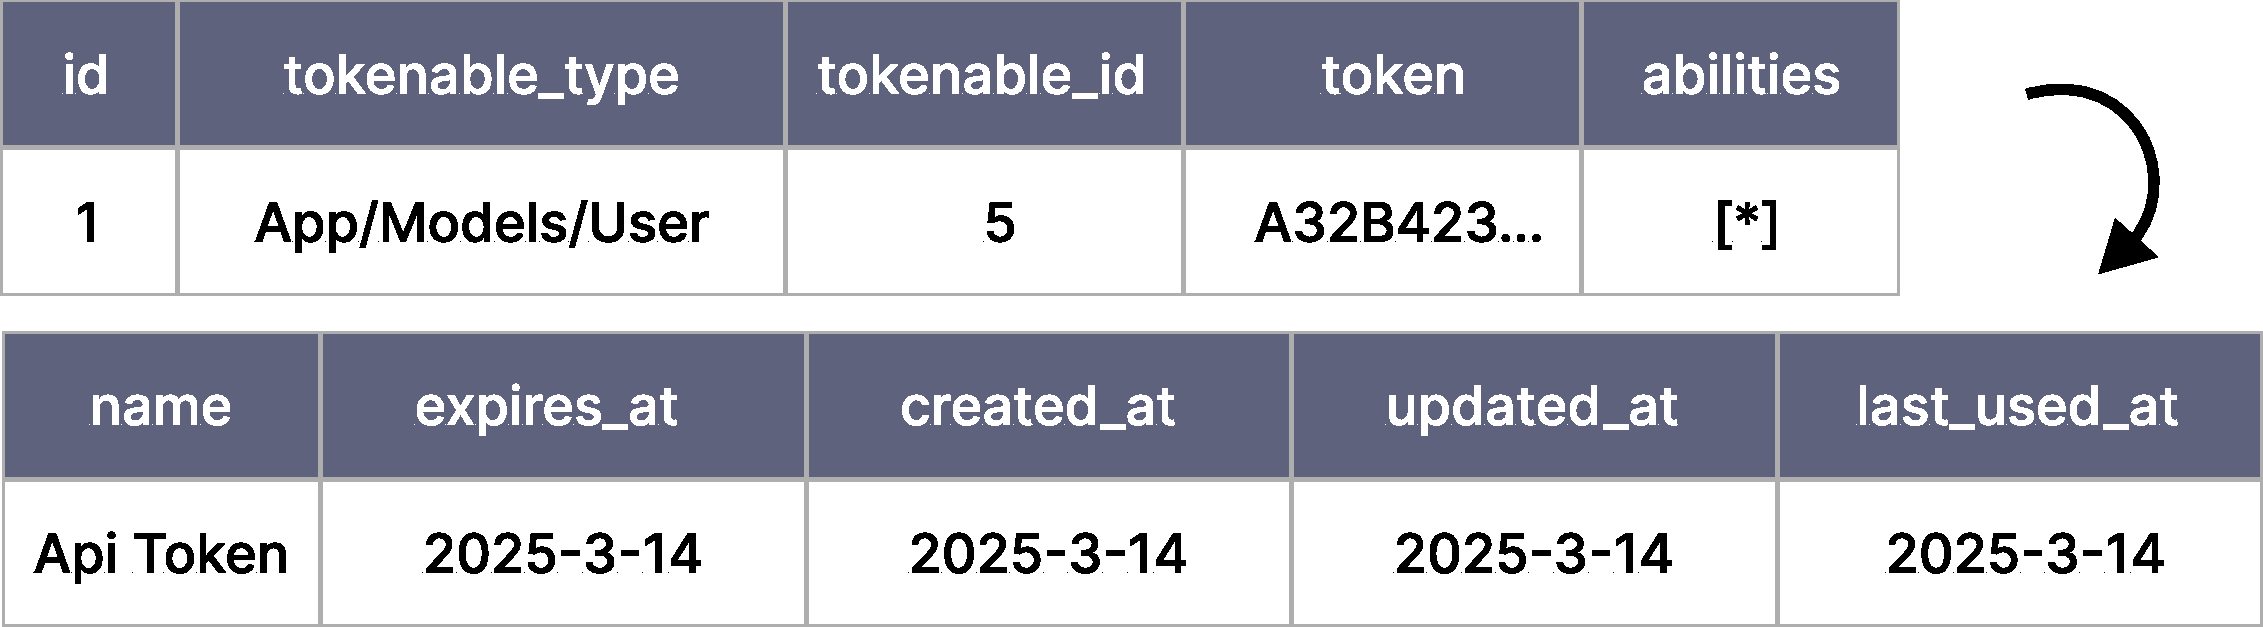
\includegraphics[width=0.9\textwidth]{images/sanctum_table@2x.pdf}
\end{figure}
\begin{center}
	\textbf{\textit{Figure: Sanctum Validation Table Schema}}
\end{center}

\begin{figure}[H]
	\centering
	\hspace*{-0.9cm}
	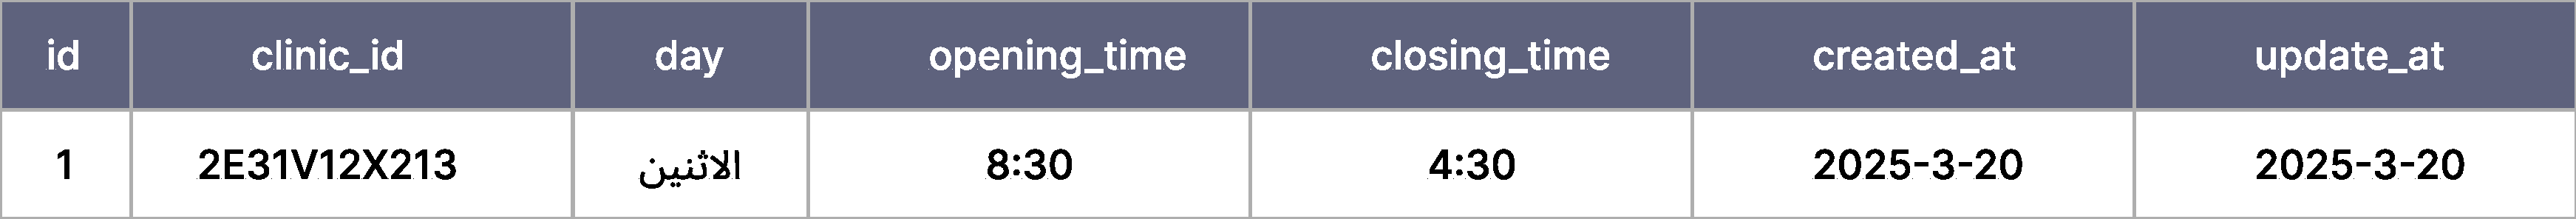
\includegraphics[width=1.1\textwidth]{images/schedule_table@2x.pdf}
\end{figure}
\begin{center}
	\textbf{\textit{Figure: Schedule Table Schema}}
\end{center}

\subsubsection*{• 2.3.5 Final Setup}
\addcontentsline{toc}{subsubsection}{2.3.5 Final Setup}
To finalize setup, we used the following command:

\begin{lstlisting}[style=darkbash, language=bash, caption={Laravel command to run migrations and seeders}, belowcaptionskip=10pt]
	php artisan migrate --seed
\end{lstlisting}
	

\noindent This command runs all migrations and executes seeders, preparing the database for integration.

\section*{3 Application's interfaces}
\addcontentsline{toc}{section}{3 Application's interfaces}
In this section, we will present the main interfaces of our application. The app is designed to be user-friendly and intuitive, ensuring a smooth experience for all users types .

\subsection*{3.1 User Interface}
\addcontentsline{toc}{subsection}{3.1 User Interface}
\vspace{0.5cm}

\begin{center}
	\begin{tabular}{c@{\hspace{4cm}}c}
		\begin{minipage}{0.31\textwidth}
			\includegraphics[width=\linewidth]{images/userApp.pdf}
			\centering \small Caption 1
		\end{minipage} &
		\begin{minipage}{0.31\textwidth}
			\includegraphics[width=\linewidth]{images/userApp.pdf}
			\centering \small Caption 2
		\end{minipage} \\
		\noalign{\vspace{1.7cm}}
		\begin{minipage}{0.31\textwidth}
			\includegraphics[width=\linewidth]{images/userApp.pdf}
			\centering \small Caption 3
		\end{minipage} &
		\begin{minipage}{0.31\textwidth}
			\includegraphics[width=\linewidth]{images/userApp.pdf}
			\centering \small Caption 4
		\end{minipage} \\
	\end{tabular}
	\end{center}
\newpage
\begin{center}
	\begin{tabular}{c@{\hspace{4cm}}c}
		\begin{minipage}{0.31\textwidth}
			\includegraphics[width=\linewidth]{images/userApp.pdf}
			\centering \small Caption 1
		\end{minipage} &
		\begin{minipage}{0.31\textwidth}
			\includegraphics[width=\linewidth]{images/userApp.pdf}
			\centering \small Caption 2
		\end{minipage} \\
		\noalign{\vspace{1.7cm}}
		\begin{minipage}{0.31\textwidth}
			\includegraphics[width=\linewidth]{images/userApp.pdf}
			\centering \small Caption 3
		\end{minipage} &
		\begin{minipage}{0.31\textwidth}
			\includegraphics[width=\linewidth]{images/userApp.pdf}
			\centering \small Caption 4
		\end{minipage} \\
	\end{tabular}
	\end{center}
\newpage
\subsection*{3.2 Admin Interface}
\addcontentsline{toc}{subsection}{3.2 Admin Interface}
\vspace{0.5cm}

\begin{center}
	\begin{tabular}{c@{\hspace{4cm}}c}
		\begin{minipage}{0.31\textwidth}
			\includegraphics[width=\linewidth]{images/adminApp.pdf}
			\centering \small Caption 1
		\end{minipage} &
		\begin{minipage}{0.31\textwidth}
			\includegraphics[width=\linewidth]{images/adminApp.pdf}
			\centering \small Caption 2
		\end{minipage} \\
		\noalign{\vspace{1.7cm}}
		\begin{minipage}{0.31\textwidth}
			\includegraphics[width=\linewidth]{images/adminApp.pdf}
			\centering \small Caption 3
		\end{minipage} &
		\begin{minipage}{0.31\textwidth}
			\includegraphics[width=\linewidth]{images/adminApp.pdf}
			\centering \small Caption 4
		\end{minipage} \\
	\end{tabular}
	\end{center}
\newpage
\begin{center}
	\begin{tabular}{c@{\hspace{4cm}}c}
		\begin{minipage}{0.31\textwidth}
			\includegraphics[width=\linewidth]{images/adminApp.pdf}
			\centering \small Caption 1
		\end{minipage} &
		\begin{minipage}{0.31\textwidth}
			\includegraphics[width=\linewidth]{images/adminApp.pdf}
			\centering \small Caption 2
		\end{minipage} \\
		\noalign{\vspace{1.7cm}}
		\begin{minipage}{0.31\textwidth}
			\includegraphics[width=\linewidth]{images/adminApp.pdf}
			\centering \small Caption 3
		\end{minipage} &
		\begin{minipage}{0.31\textwidth}
			\includegraphics[width=\linewidth]{images/adminApp.pdf}
			\centering \small Caption 4
		\end{minipage} \\
	\end{tabular}
	\end{center}

	\newpage
	\subsection*{3.3 Clinic Interface}
	\addcontentsline{toc}{subsection}{3.3 Clinic Interface}
	\vspace{0.5cm}
	
	\begin{center}
		\begin{tabular}{c@{\hspace{4cm}}c}
			\begin{minipage}{0.31\textwidth}
				\includegraphics[width=\linewidth]{images/clinicApp.pdf}
				\centering \small Caption 1
			\end{minipage} &
			\begin{minipage}{0.31\textwidth}
				\includegraphics[width=\linewidth]{images/clinicApp.pdf}				
				\centering \small Caption 2
			\end{minipage} \\
			\noalign{\vspace{1.7cm}}
			\begin{minipage}{0.31\textwidth}
				\includegraphics[width=\linewidth]{images/clinicApp.pdf}				
				\centering \small Caption 3
			\end{minipage} &
			\begin{minipage}{0.31\textwidth}
				\includegraphics[width=\linewidth]{images/clinicApp.pdf}
				\centering \small Caption 4
			\end{minipage} \\
		\end{tabular}
		\end{center}
	\newpage
	\begin{center}
		\begin{tabular}{c@{\hspace{4cm}}c}
			\begin{minipage}{0.31\textwidth}
				\includegraphics[width=\linewidth]{images/clinicApp.pdf}
				\centering \small Caption 1
			\end{minipage} &
			\begin{minipage}{0.31\textwidth}
				\includegraphics[width=\linewidth]{images/clinicApp.pdf}
				\centering \small Caption 2
			\end{minipage} \\
			\noalign{\vspace{1.7cm}}
			\begin{minipage}{0.31\textwidth}
				\includegraphics[width=\linewidth]{images/clinicApp.pdf}
				\centering \small Caption 3
			\end{minipage} &
			\begin{minipage}{0.31\textwidth}
				\includegraphics[width=\linewidth]{images/clinicApp.pdf}
				\centering \small Caption 4
			\end{minipage} \\
		\end{tabular}
		\end{center}
	
		\newpage
\subsection*{3.4 Doctor Interface}
\addcontentsline{toc}{subsection}{3.4 Doctor Interface}
\vspace{0.5cm}

\begin{center}
	\begin{tabular}{c@{\hspace{4cm}}c}
		\begin{minipage}{0.31\textwidth}
			\includegraphics[width=\linewidth]{images/doctorApp.pdf}
			\centering \small Caption 1
		\end{minipage} &
		\begin{minipage}{0.31\textwidth}
			\includegraphics[width=\linewidth]{images/doctorApp.pdf}
			\centering \small Caption 2
		\end{minipage} \\
		\noalign{\vspace{1.7cm}}
		\begin{minipage}{0.31\textwidth}
			\includegraphics[width=\linewidth]{images/doctorApp.pdf}
			\centering \small Caption 3
		\end{minipage} &
		\begin{minipage}{0.31\textwidth}
			\includegraphics[width=\linewidth]{images/doctorApp.pdf}
			\centering \small Caption 4
		\end{minipage} \\
	\end{tabular}
	\end{center}
\newpage
\begin{center}
	\begin{tabular}{c@{\hspace{4cm}}c}
		\begin{minipage}{0.31\textwidth}
			\includegraphics[width=\linewidth]{images/doctorApp.pdf}
			\centering \small Caption 1
		\end{minipage} &
		\begin{minipage}{0.31\textwidth}
			\includegraphics[width=\linewidth]{images/doctorApp.pdf}
			\centering \small Caption 2
		\end{minipage} \\
		\noalign{\vspace{1.7cm}}
		\begin{minipage}{0.31\textwidth}
			\includegraphics[width=\linewidth]{images/doctorApp.pdf}
			\centering \small Caption 3
		\end{minipage} &
		\begin{minipage}{0.31\textwidth}
			\includegraphics[width=\linewidth]{images/doctorApp.pdf}
			\centering \small Caption 4
		\end{minipage} \\
	\end{tabular}
	\end{center}


\newpage
\section*{4 Conclusion}
\addcontentsline{toc}{section}{4 Conclusion}

\noindent In this chapter, we provided a comprehensive overview of the technical implementation of our mobile application. 

\vspace{0.3cm}

\noindent We detailed the hardware and software environments, explained the selection of technologies, and outlined the database architecture and authentication mechanisms. 

\vspace{0.3cm}

\noindent By presenting key code snippets, diagrams, and database schemas, we offered a clear view of the internal workings that ensure the app’s functionality, security, and user experience. 

\vspace{0.3cm}

\noindent This practical insight serves as a foundation for understanding how the various components of our system come together to deliver a robust and scalable solution.


\newpage
\begin{center}
	\Huge \textbf{General Conclusion} \\
	\addcontentsline{toc}{chapter}{General Conclusion}
	\vspace*{0.3cm}
\end{center}

\noindent In conclusion, this work has made it possible to \textbf{design}, \textbf{develop}, and \textbf{deploy} a functional mobile application, integrating \textbf{modern technologies} and \textbf{effective development practices}.

\vspace{0.3cm}

\noindent Thanks to a \textbf{rigorous approach}, we were able to ensure a \textbf{smooth}, \textbf{secure}, and \textbf{user-friendly experience} that meets the identified needs.

\vspace{0.3cm}

\noindent The \textbf{challenges} encountered throughout the project were valuable \textbf{opportunities for learning and improvement}, helping to strengthen both our \textbf{technical} and \textbf{organizational skills}.

\vspace{0.3cm}

\noindent This project provides a \textbf{solid foundation} for future \textbf{enhancements} and \textbf{evolutions}. We fully intend to \textbf{continue improving the application}, adding new \textbf{features}, refining existing functionalities, and incorporating user feedback to ensure the app remains \textbf{innovative}, \textbf{relevant}, and aligned with evolving user expectations.


\vspace{1cm}

\newpage
\addcontentsline{toc}{chapter}{Bibliographie}

\begin{thebibliography}{18}
    \bibitem{flutter} Flutter Documentation, \textit{\url{https://flutter.dev/docs}}
    \bibitem{laravel} Laravel Documentation, \textit{\url{https://laravel.com/docs}}
    \bibitem{mysql} MySQL Documentation, \textit{\url{https://dev.mysql.com/doc/}}
    \bibitem{firebase} Firebase Documentation, \textit{\url{https://firebase.google.com/docs}}
    \bibitem{github} GitHub Guides, \textit{\url{https://guides.github.com}}
    \bibitem{figma} Figma Help Center, \textit{\url{https://help.figma.com}}
    \bibitem{googlemap} Google Maps Platform Documentation, \textit{\url{https://developers.google.com/maps/documentation}}
    \bibitem{php} PHP Manual, \textit{\url{https://www.php.net/manual/en/}}
    \bibitem{vscode} Visual Studio Code Docs, \textit{\url{https://code.visualstudio.com/docs}}
    \bibitem{androidstudio} Android Studio User Guide, \textit{\url{https://developer.android.com/studio}}
    \bibitem{postman} Postman Learning Center, \textit{\url{https://learning.postman.com}}
    \bibitem{dbdiagram} dbdiagram.io Documentation, \textit{\url{https://dbdiagram.io/docs}}
    \bibitem{sanctum} Laravel Sanctum Documentation, \textit{\url{https://laravel.com/docs/sanctum}}
    \bibitem{git} Git Documentation, \textit{\url{https://git-scm.com/doc}}
    \bibitem{hostinger} Hostinger Tutorials, \textit{\url{https://www.hostinger.com/tutorials}}
    \bibitem{fluttermap} Flutter Map Package, \textit{\url{https://pub.dev/packages/flutter_map}}
    \bibitem{mvcflutter} Faiz Rahmat, “Understanding MVC Architecture in Flutter: A Comprehensive Guide with Examples,” Medium, \textit{\url{https://medium.com/@Faiz_Rhm/understanding-mvc-architecture-in-flutter-a-comprehensive-guide-with-examples-5d1a372c7eaf}}
    \bibitem{mvclaravel} Laravel and MVC Framework, GeeksforGeeks, \textit{\url{https://www.geeksforgeeks.org/introduction-to-laravel-and-mvc-framework/}}
\end{thebibliography}

	

\end{document}